% parity_tournaments_extended.tex
% Extended version: incorporates all content from proof-status documents.
% New material: Claim A/B scaffold with full proof of Claim B, per-path identity,
% ins_act theorem, proof strategies for Claim A, corrected pair counts,
% expanded counterexample, updated verification tables, and new open problems.
% Compile: pdflatex parity_tournaments_extended.tex  (twice for cross-refs)
\documentclass[12pt,reqno]{amsart}
\usepackage[margin=1.25in,top=1.1in,bottom=1.2in]{geometry}

%─── Encoding & typography ────────────────────────────────────────────────────
\usepackage[T1]{fontenc}
\usepackage[utf8]{inputenc}
\usepackage[protrusion=true,expansion=false]{microtype}

%─── Math ─────────────────────────────────────────────────────────────────────
\usepackage{amsmath,amssymb,amsthm,mathtools}
\allowdisplaybreaks

%─── Layout & tables ──────────────────────────────────────────────────────────
\usepackage{enumitem}
\usepackage{booktabs,array,tabularx}
\usepackage{multicol}
\usepackage[font=small,labelfont=bf]{caption}
\usepackage[section]{placeins}

%─── Graphics & TikZ ──────────────────────────────────────────────────────────
\usepackage{graphicx}
\usepackage{tikz}
\usetikzlibrary{%
  positioning,calc,decorations.pathreplacing,
  arrows.meta,patterns,shapes.geometric,
  matrix,backgrounds,fit,shapes.multipart}

%─── Boxes & color ────────────────────────────────────────────────────────────
\usepackage{xcolor}
\usepackage{mdframed}
\usepackage{tcolorbox}
\tcbuselibrary{skins,breakable,theorems}

%─── Code listings ────────────────────────────────────────────────────────────
\usepackage{listings}
\usepackage{pifont}
\newcommand{\cmark}{\ding{51}}
\newcommand{\xmark}{\ding{55}}

%─── Colors ───────────────────────────────────────────────────────────────────
\definecolor{inkblue}{RGB}{20,50,140}
\definecolor{axisblue}{RGB}{25,70,190}
\definecolor{axisred}{RGB}{185,30,30}
\definecolor{axisteal}{RGB}{0,125,115}
\definecolor{tilefix}{RGB}{160,195,245}
\definecolor{tilerot1}{RGB}{255,215,130}
\definecolor{tilerot2}{RGB}{190,235,190}
\definecolor{tileborder}{RGB}{80,80,110}
\definecolor{openred}{RGB}{155,25,25}
\definecolor{proofblue}{RGB}{25,55,140}
\definecolor{depbg}{RGB}{237,246,255}
\definecolor{depborder}{RGB}{150,190,230}
\definecolor{highlightbg}{RGB}{255,251,235}
\definecolor{highlightborder}{RGB}{200,175,80}
\definecolor{sketchbg}{RGB}{245,248,255}
\definecolor{routeAbg}{RGB}{240,255,240}
\definecolor{routeBbg}{RGB}{255,250,240}
\definecolor{routeCbg}{RGB}{240,244,255}
\definecolor{routeDbg}{RGB}{248,240,255}
\definecolor{contribbox}{RGB}{235,243,255}
\definecolor{resolvedgreen}{RGB}{0,120,60}
\definecolor{claimAbg}{RGB}{255,245,245}
\definecolor{claimBbg}{RGB}{245,255,245}
\definecolor{perpathbg}{RGB}{250,248,240}

%─── Hyperlinks ───────────────────────────────────────────────────────────────
\usepackage{hyperref}
\hypersetup{
  colorlinks=true,
  linkcolor=proofblue,
  citecolor=proofblue,
  urlcolor=axisteal,
  pdftitle={Parity in Tournaments: The Q-Lemma, the Tiling Model, and the Odd-Cycle Collection Formula},
  pdfauthor={},
  pdfsubject={Combinatorics, Tournaments, Redei's Theorem},
  pdfkeywords={tournament, Hamiltonian path, parity, tiling model, odd-cycle collection formula},
}
\usepackage[capitalise,nameinlink]{cleveref}

%═══════════════════════════════════════════════════════
%  THEOREM ENVIRONMENTS
%═══════════════════════════════════════════════════════
\theoremstyle{plain}
\newtheorem{theorem}{Theorem}[section]
\newtheorem{lemma}[theorem]{Lemma}
\newtheorem{proposition}[theorem]{Proposition}
\newtheorem{corollary}[theorem]{Corollary}

\theoremstyle{definition}
\newtheorem{definition}[theorem]{Definition}
\newtheorem{example}[theorem]{Example}

\theoremstyle{remark}
\newtheorem{remark}[theorem]{Remark}
\newtheorem{conjecture}[theorem]{Conjecture}
\newtheorem{openquestion}[theorem]{Open Problem}

%═══════════════════════════════════════════════════════
%  TCOLORBOX ENVIRONMENTS
%═══════════════════════════════════════════════════════
\tcbset{
  routebox/.style={
    enhanced, breakable,
    colback=#1!8, colframe=#1!60!black,
    fonttitle=\bfseries\small, coltitle=white,
    colbacktitle=#1!60!black,
    attach title to upper={\par\smallskip},
    left=4pt, right=4pt, top=4pt, bottom=4pt,
    sharp corners=south
  }
}

\newtcolorbox{depbox}{
  enhanced, breakable,
  colback=depbg, colframe=depborder,
  boxrule=1pt, arc=3pt,
  left=8pt, right=8pt, top=8pt, bottom=6pt,
  title={\textbf{\textsf{Route Dependency Summary (no circular reasoning)}}},
  fonttitle=\bfseries\small, coltitle=white,
  colbacktitle=inkblue,
  titlerule=0pt, toptitle=3pt, bottomtitle=3pt,
}

\newtcolorbox{highlightbox}[1][]{
  enhanced,
  colback=highlightbg, colframe=highlightborder,
  boxrule=1.5pt, arc=2pt,
  left=8pt, right=8pt, top=6pt, bottom=6pt,
  #1
}

\newtcolorbox{sketchbox}[1][]{
  enhanced, breakable,
  colback=sketchbg, colframe=inkblue!40,
  boxrule=0.8pt, arc=2pt,
  left=6pt, right=6pt, top=4pt, bottom=4pt,
  fonttitle=\bfseries\small, coltitle=black,
  colbacktitle=inkblue!10,
  titlerule=0.4pt, toptitle=2pt, bottomtitle=2pt,
  #1
}

\newtcolorbox{contribbox}{
  enhanced,
  colback=contribbox, colframe=inkblue!50,
  boxrule=1pt, arc=3pt,
  left=8pt, right=8pt, top=8pt, bottom=6pt,
  boxsep=0pt,
  title={\textbf{\textsf{New Contributions}}},
  fonttitle=\bfseries\small, coltitle=white,
  colbacktitle=inkblue,
  titlerule=0pt, toptitle=3pt, bottomtitle=3pt,
}

\newtcolorbox{correctionbox}[1][]{
  enhanced,
  colback=red!4, colframe=red!50!black,
  boxrule=1pt, arc=3pt,
  left=8pt, right=8pt, top=6pt, bottom=6pt,
  width=\linewidth,
  title={\textbf{\textsf{Note}}},
  fonttitle=\bfseries\small, coltitle=white,
  colbacktitle=red!50!black,
  #1
}

\newtcolorbox{claimAbox}{
  enhanced, breakable,
  colback=claimAbg, colframe=axisred!60,
  boxrule=1.2pt, arc=3pt,
  left=8pt, right=8pt, top=6pt, bottom=6pt,
  width=\linewidth,
  title={\textbf{\textsf{Claim A --- Central Open Problem}}},
  fonttitle=\bfseries\small, coltitle=white,
  colbacktitle=axisred!70,
  titlerule=0pt, toptitle=3pt, bottomtitle=3pt,
}

\newtcolorbox{claimBbox}{
  enhanced, breakable,
  colback=claimBbg, colframe=axisteal!60,
  boxrule=1.2pt, arc=3pt,
  left=8pt, right=8pt, top=6pt, bottom=6pt,
  width=\linewidth,
  title={\textbf{\textsf{Claim B --- Proved}}},
  fonttitle=\bfseries\small, coltitle=white,
  colbacktitle=axisteal!80,
  titlerule=0pt, toptitle=3pt, bottomtitle=3pt,
}

\newtcolorbox{perpathbox}{
  enhanced, breakable,
  colback=perpathbg, colframe=inkblue!50,
  boxrule=1pt, arc=3pt,
  left=8pt, right=8pt, top=6pt, bottom=6pt,
}

%═══════════════════════════════════════════════════════
%  CODE LISTINGS
%═══════════════════════════════════════════════════════
\lstdefinestyle{pythoncode}{
  language=Python,
  basicstyle=\ttfamily\footnotesize,
  keywordstyle=\color{blue!70!black}\bfseries,
  stringstyle=\color{green!50!black},
  commentstyle=\color{gray!70}\itshape,
  numberstyle=\tiny\color{gray},
  frame=single, framesep=4pt,
  numbers=left, numbersep=8pt,
  breaklines=true, showstringspaces=false,
  tabsize=4, backgroundcolor=\color{gray!6},
  rulecolor=\color{gray!40}, captionpos=b,
  xleftmargin=12pt, xrightmargin=4pt,
}
\lstset{style=pythoncode}

%─── Macros ───────────────────────────────────────────────────────────────────
\DeclareMathOperator{\Aut}{Aut}
\DeclareMathOperator{\Fix}{Fix}
\DeclareMathOperator{\Grid}{Grid}
\DeclareMathOperator{\Str}{Str}  % used in Definition~\ref{def:grid} for strips
\newcommand{\Ham}{\mathrm{Ham}}
\newcommand{\id}{\mathrm{id}}
\newcommand{\op}{\mathrm{op}}
\newcommand{\ZZ}{\mathbb{Z}}
\newcommand{\indthree}{\mathbf{1}_{3\mid n}}
\newcommand{\iverson}[1]{\bigl[\,#1\,\bigr]}
\newcommand{\routeA}{\textcolor{axisteal}{\textbf{Route~A}}}
\newcommand{\routeB}{\textcolor{axisred}{\textbf{Route~B}}}
\newcommand{\routeC}{\textcolor{inkblue}{\textbf{Route~C}}}
\newcommand{\routeD}{\textcolor{axisteal!80!black}{\textbf{Route~D}}}
\newcommand{\inshat}{\widehat{\mathrm{ins}}}
\newcommand{\insact}{\mathrm{ins}_{\mathrm{act}}}

\pdfstringdefDisableCommands{%
  \renewcommand{\ZZ}{Z}%
  \renewcommand{\indthree}{1[3|n]}%
  \renewcommand{\Ham}{Ham}%
  \renewcommand{\routeA}{Route A}%
  \renewcommand{\routeB}{Route B}%
  \renewcommand{\routeC}{Route C}%
  \renewcommand{\routeD}{Route D}%
  \renewcommand{\inshat}{ins-hat}%
  \renewcommand{\insact}{ins-act}%
}

\renewcommand{\qedsymbol}{$\blacksquare$}

%═══════════════════════════════════════════════════════
%  TITLE BLOCK
%═══════════════════════════════════════════════════════
\title[Parity in Tournaments]{%
  Parity in Tournaments:\\[4pt]
  The Q-Lemma, the Tiling Model,\\[2pt]
  and the Odd-Cycle Collection Formula}

\date{March 2026}

\begin{document}

\begin{abstract}
We introduce a \emph{tiling model} encoding every $n$-vertex tournament as a
binary assignment on a triangular \emph{pin grid} $\Grid(n) \cong \delta_{n-2}$,
making lattice symmetries correspond to arc-reversal involutions.
Using this model we give four independent proofs of R\'{e}dei's theorem
($H(T)$ odd for every tournament $T$): a fixed-point-free involution on
two-block path decompositions (the \textbf{Q-Lemma}, \textbf{Route~A},
conditional on the per-3-cycle parity conjecture, verified exhaustively for
$n\le4$),
a $\beta$-involution reduction to a smaller tournament (\textbf{Route~B}),
a free automorphism-group action (\textbf{Route~C}, unconditional), and the
\emph{Odd-Cycle Collection Formula} (\textbf{Route~D}):
\[
  H(T) = I(\Omega(T),\,2),
\]
where $\Omega(T)$ is the conflict graph of directed odd cycles of $T$ and
$I(G,x)$ is the independence polynomial.
The OCF was proved by Grinberg and Stanley~\cite{grinberg2024} via
$P$-partition theory; we give an independent elementary proof via
Walsh--Fourier analysis.

The algebraic half of the OCF induction
(\textbf{Claim~B}: $I(\Omega(T),2)-I(\Omega(T{-}v),2)=2\sum_{C\ni v}\mu(C)$,
where $\mu(C)$ is the independence polynomial at~$2$ of the conflict graph
restricted to odd cycles disjoint from $C\setminus\{v\}$) is proved via
an $A$-clique argument. The combinatorial half (\textbf{Claim~A}:
$H(T)-H(T{-}v)=2\sum_{C\ni v}\mu(C)$) is proved by
Grinberg--Stanley~\cite{grinberg2024};
it was verified exhaustively for $n\le 6$ (196,608 pairs) and by random
sampling at $n=7$ (3,500 pairs, zero failures) before the proof appeared.
A \emph{per-path identity} implies Claim~A for $n\le5$ (where all odd cycles
through $v$ are 3-cycles) but fails at $n=6$ due to 5-cycles.
We also give the first purely combinatorial proof of Forcade's
$\mathbb{F}_2$-invariance for all $k$-block decompositions, prove closed-form
$S_3\times\mathbb{Z}_2$ orbit counts for the pin grid (with proofs via
Burnside's lemma and barycentric coordinates), show that all hook lengths
of $\delta_{n-2}$ are odd, and identify the self-evacuating SYT count with
$|\mathrm{Fix}(\sigma)|=2^{m^2}$ for $n=2m+1$ (verified for $n=5,7$;
full proof conditional on a precise classical reference).
A complete proof-status table distinguishes all proved, refuted, open, and
verified-but-unproved claims.
\end{abstract}

\maketitle
\setcounter{tocdepth}{2}
\tableofcontents

%═══════════════════════════════════════════════════════════════════════════════
\section{Introduction}
\label{sec:intro}
%═══════════════════════════════════════════════════════════════════════════════

A \emph{tournament} $T$ on vertex set $V=\{1,\ldots,n\}$ is a complete directed
graph: for every pair $\{u,v\}\subset V$, exactly one of $u\to v$ or $v\to u$
holds. We encode this by $T(u,v)=1$ if $u\to v$, with $T(u,v)+T(v,u)=1$ for all
$u\ne v$. Write $H(T)$ for the number of directed Hamiltonian paths in $T$.

\begin{theorem}[Rédei, 1934 \cite{redei1934}]\label{thm:redei}
$H(T)\equiv 1\pmod{2}$ for every tournament $T$.
\end{theorem}

\noindent Every tournament has an \emph{odd} number of Hamiltonian paths.
This paper makes the combinatorial structure behind this result explicit through
four independent proof routes, a detailed study of the pin grid geometry, and a
complete 2-adic refinement via the Odd-Cycle Collection Formula.

\subsection{The pin grid}

Fix the \emph{base path} $P_0\colon n\to n{-}1\to\cdots\to 1$. A tournament
containing $P_0$ is determined by the orientation of all \emph{non-path arcs}
$(a,b)$ with $a\ge b+2$. There are $m=\binom{n-1}{2}$ such pairs. Assign
coordinate $(r,c)$ by $r:=a-b-1\ge 1$, $c:=b\ge 1$; this produces the
\emph{pin grid}
\[
  \Grid(n) := \{(r,c)\in\mathbb{Z}^2 : r\ge 1,\; c\ge 1,\; r+c\le n-1\},
\]
isomorphic to the staircase Young diagram $\delta_{n-2}$. A \emph{tiling}
$t\in\{0,1\}^m$ assigns a bit to each tile: bit $0$ means $a\to b$ and bit
$1$ means $b\to a$.

\subsection{The Odd-Cycle Collection Formula and Claim A}

The main combinatorial formula of this paper is:

\begin{theorem}[Odd-Cycle Collection Formula {\cite{grinberg2024}}]\label{thm:ocf_main}
For every tournament $T$ on $n$ vertices:
\[
  H(T) = I(\Omega(T),\,2) = \sum_{k\geq 0} \alpha_k(\Omega(T))\cdot 2^k,
\]
where $\Omega(T)$ is the conflict graph on directed odd cycles of $T$ (vertices
are odd cycles, edges connect pairs sharing a vertex), $I(G,x)$ is the
independence polynomial of $G$, and $\alpha_k$ counts independent sets of
size $k$.
\end{theorem}

The formula was computationally verified exhaustively for all $n \leq 6$ and by
random sampling at $n = 7$ before being proved by Grinberg and
Stanley~\cite{grinberg2024}. The inductive proof structure reduces to
\textbf{Claim~A} (see \S\ref{sec:ocf}), which is now established.

\subsection{Verification record}
\label{subsec:verification_record}

All computations below were independently rerun. The pair counts refer to
$(T, v)$ pairs (tournaments times vertices). At $n=4$ there are
$2^{\binom{4}{2}} = 64$ tournaments, giving $64 \times 4 = 256$ pairs $(T,v)$;
all failure counts below are over these 256 pairs.

\begin{center}
\footnotesize\renewcommand{\arraystretch}{1.18}
\begin{tabular}{p{5.6cm} c c c c}
\toprule
\textbf{Claim / Test} & \textbf{$n=4$} & \textbf{$n=5$} & \textbf{$n=6$} & \textbf{$n=7$}\\
& (256 pairs) & (5,120) & (196,608) & (3,500 rnd)\\
\midrule
Claim~A: $H(T)-H(T{-}v) = 2\sum\mu(C)$ & 0 fails & 0 fails & 0 fails \checkmark & 0 fails \checkmark\\
Claim~B: $I(\Omega,2)-I(\Omega{-}v,2) = 2\sum\mu(C)$ & 0 fails & 0 fails & 0 fails \checkmark & ---\\
$H(T) \equiv B_v+S_v+R_v \pmod{2}$ & 0 fails & --- & --- & ---\\
$H(T) = B_v+S_v+R_v$ (exact) & \textbf{96 fails} $\times$ & --- & --- & ---\\
$S_v+R_v = 2\sum\mu(C)$ & \textbf{144 fails} $\times$ & --- & --- & ---\\
$\insact(v,P')=B_v(P')+S_v(P')$ per path & 0 fails & 0 fails & 0 fails \checkmark & ---\\
$\inshat(v,P')$ always odd & 0 fails & 0 fails & 0 fails \checkmark & ---\\
$\sum_{P'}\insact(v,P') = H(T)$ & \textbf{96 fails} $\times$ & --- & --- & ---\\
Per-path identity (3-cycle case) & --- & 0 fails & \textbf{2,758/9,126} $\times$ & ---\\
\bottomrule
\end{tabular}
\end{center}

\subsection{Main contributions}

\noindent\begin{contribbox}
\begin{enumerate}[label=\textbf{\arabic*.},leftmargin=1.4em,itemsep=4pt]
  \item \textbf{The tiling model.} A bijection between $\{0,1\}^m$ and
    labeled $n$-vertex tournaments equipped with a fixed base path $P_0$,
    making the $S_3$ and $\mathbb{Z}_2$ symmetries of the pin grid $\Grid(n)$
    transparent as arc-reversal involutions.
  \item \textbf{The Q-Lemma (\routeA).} A self-contained cyclic-cut parity
    proof of Rédei's theorem conditional on the per-3-cycle parity conjecture
    (Conjecture~\ref{lem:per_cycle_parity}, verified for $n\le4$). The
    Q-Lemma involution itself (Lemma~\ref{lem:toggle}) is unconditional and
    is the $k=2$ case of Forcade's
    $\mathbb{F}_2$-invariance \cite{forcade1973}, proved here purely
    combinatorially.
  \item \textbf{The Forcade Generalization.} The first purely combinatorial
    proof of $\mathbb{F}_2$-invariance for all $k$-block decompositions.
  \item \textbf{Claim~B proved.} The algebraic companion of Claim~A is
    proved via an $A$-clique argument on $\Omega(T)$ (\S\ref{subsec:scaffold}).
    Claim~A remains open.
  \item \textbf{The per-path identity.} A new path-by-path version of
    Claim~A, proved for $n \leq 5$, shown to fail at $n=6$ due to
    5-cycles (\S\ref{sec:perpath}).
  \item \textbf{The $\insact$ theorem.} The actual valid insertion count per
    path is $\insact(v,P') = B_v(P') + S_v(P')$, proved and verified
    (\S\ref{subsec:insact}).
  \item \textbf{Proof strategies for Claim~A.} Five organized approaches
    toward proving the central open problem (\S\ref{subsec:claim_strategies}).
  \item \textbf{OCF formula and 2-adic tower.} The exact formula
    $H(T)=I(\Omega(T),2)$; higher-order Rédei theorems; connection to
    the hard-core lattice gas at fugacity~2.
  \item \textbf{$S_3\times\mathbb{Z}_2$ analysis of the pin grid.}
    Closed-form fixed-tiling counts, Burnside orbit formula, all-odd hook
    lengths of $\delta_{n-2}$, TSSCPP identification.
\end{enumerate}
\end{contribbox}

\subsection{Organization}

Sections~\ref{sec:setup}--\ref{sec:routeC} build the tiling model and give
Routes~A--C. \textbf{Section~\ref{sec:ocf}} is the central new section: it develops the
deletion-vertex scaffold (Claims~A and~B), the $\mu(C)$ notation, the per-path
identity, and organized proof strategies for Claim~A.
Section~\ref{sec:S3} develops the $S_3$ geometry.
Section~\ref{sec:classes} gives the double-Burnside formula.
Section~\ref{sec:tetra} covers Young diagrams and TSSCPPs.
Section~\ref{sec:literature} discusses related work.
Section~\ref{sec:resolved} gives complete proofs of resolved problems and
corrects errors. Section~\ref{sec:open} lists remaining open problems.

%═══════════════════════════════════════════════════════════════════════════════
\section{Setup and the Pin Grid}
\label{sec:setup}
%═══════════════════════════════════════════════════════════════════════════════

\subsection{Tournaments and the tiling encoding}

Set $T(u,v)=1$ for $u\to v$, with $T(u,v)+T(v,u)=1$ for all $u\ne v\in V$.
The \emph{opposite tournament} $T^{\op}$ reverses all arcs: $T^{\op}(u,v)=T(v,u)$.
An \emph{anti-automorphism} of $T$ is a bijection $\alpha:V\to V$ with
$T(\alpha(u),\alpha(v))=T(v,u)$.

\begin{definition}[Tiling encoding]\label{def:tiling}
Fix the \emph{base path} $P_0\colon n\to n{-}1\to\cdots\to 1$. A \emph{tile}
is a pair $(a,b)$ with $a,b\in V$ and $a\ge b+2$; $m=\binom{n-1}{2}$. In
coordinates $a=r+c+1$, $b=c$, a \emph{tiling} $t\in\{0,1\}^m$ assigns: bit
$0$ means $a\to b$ (forward); bit $1$ means $b\to a$ (backward). This determines
a unique tournament $T_t$ containing $P_0$.
\end{definition}

\begin{proposition}[Transitive tournament]
\label{prop:transitive}
The all-zero tiling gives the transitive tournament with $H=1$; the all-one
tiling gives its opposite, also $H=1$. Moreover $H(T)=1$ iff $T$ is transitive.
\end{proposition}
\begin{proof}
The transitive tournament on $\{1,\ldots,n\}$ has $i\to j$ iff $i>j$. The unique
Hamiltonian path is $n\to n{-}1\to\cdots\to 1 = P_0$; any other ordering fails at some step.
Conversely, if $T$ is not transitive, it contains a directed 3-cycle
$a\to b\to c\to a$, so $\alpha_1(\Omega(T)) \geq 1$. By the OCF
(Theorem~\ref{thm:ocf_main}), $H(T) = 1 + 2\alpha_1 + 4\alpha_2 + \cdots
\geq 1 + 2 = 3 > 1$.
\end{proof}

\subsection{The pin grid and canonical coordinates}

\begin{definition}[Pin grid]\label{def:grid}
\[
  \Grid(n) := \{(r,c)\in\mathbb{Z}^2 : r\ge 1,\; c\ge 1,\; r+c\le n-1\},
\quad |\Grid(n)| = m = \binom{n-1}{2}.
\]
The \emph{strip} $\Str(k) := \{(r,c) : r+c=k,\; r,c\ge 1\}$ has $k-1$ tiles.
\end{definition}

Figure~\ref{fig:grids} illustrates $\Grid(4)$ ($m=3$ tiles) and $\Grid(5)$
($m=6$ tiles), with the $\sigma$-fixed diagonal $r=c$ highlighted.

\begin{figure}[htbp]
\centering
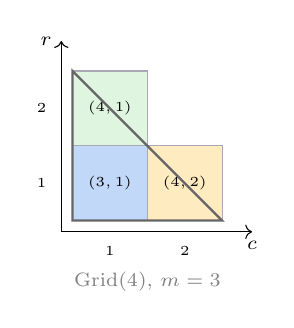
\begin{tikzpicture}[scale=0.95,baseline=(current bounding box.center)]
  \fill[tilefix!65]  (0,0) rectangle (1,1);
  \fill[tilerot1!50] (1,0) rectangle (2,1);
  \fill[tilerot2!50] (0,1) rectangle (1,2);
  \foreach \r/\c in {1/1, 1/2, 2/1}{
    \draw[tileborder!50,thin] (\c-1,\r-1) rectangle (\c,\r);
    \pgfmathtruncatemacro{\aa}{\r+\c+1}
    \node[font=\tiny] at (\c-0.5,\r-0.5) {$(\aa,\c)$};
  }
  \draw[black!60,thick] (0,0)--(2,0)--(0,2)--cycle;
  \draw[->] (-0.15,-0.15)--(-0.15,2.4) node[left,font=\scriptsize]{$r$};
  \draw[->] (-0.15,-0.15)--(2.4,-0.15) node[below,font=\scriptsize]{$c$};
  \foreach \x in {1,2} \node[below,font=\tiny] at (\x-0.5,-0.22){\x};
  \foreach \y in {1,2} \node[left, font=\tiny] at (-0.22,\y-0.5){\y};
  \node[below,font=\scriptsize,gray] at (1.0,-0.55){$\Grid(4)$, $m=3$};
\end{tikzpicture}
\qquad
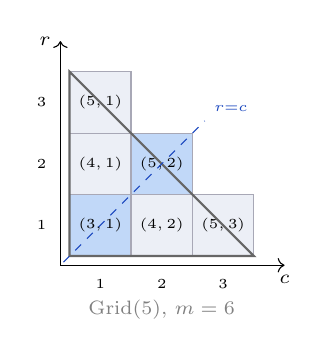
\begin{tikzpicture}[scale=0.78,baseline=(current bounding box.center)]
  \foreach \r/\c in {1/1, 1/2, 1/3, 2/1, 2/2, 3/1}{
    \pgfmathtruncatemacro{\aa}{\r+\c+1}
    \ifnum\r=\c
      \fill[tilefix!65] (\c-1,\r-1) rectangle (\c,\r);
    \else
      \fill[inkblue!8] (\c-1,\r-1) rectangle (\c,\r);
    \fi
    \draw[tileborder!50,thin] (\c-1,\r-1) rectangle (\c,\r);
    \node[font=\tiny] at (\c-0.5,\r-0.5) {$(\aa,\c)$};
  }
  \draw[black!60,thick] (0,0)--(3,0)--(0,3)--cycle;
  \draw[axisblue,dashed,thin] (-0.1,-0.1)--(2.2,2.2)
    node[above right,font=\tiny,axisblue]{$r{=}c$};
  \draw[->] (-0.15,-0.15)--(-0.15,3.5) node[left,font=\scriptsize]{$r$};
  \draw[->] (-0.15,-0.15)--(3.5,-0.15) node[below,font=\scriptsize]{$c$};
  \foreach \x in {1,2,3} \node[below,font=\tiny] at (\x-0.5,-0.22){\x};
  \foreach \y in {1,2,3} \node[left, font=\tiny] at (-0.22,\y-0.5){\y};
  \node[below,font=\scriptsize,gray] at (1.5,-0.55){$\Grid(5)$, $m=6$};
\end{tikzpicture}
\caption{Pin grids $\Grid(4)$ ($m=3$) and $\Grid(5)$ ($m=6$).
Shaded tiles lie on the $\sigma$-fixed axis $r=c$.}
\label{fig:grids}
\end{figure}

\subsection{Symmetry operations}

\begin{definition}[Grid symmetries]\label{def:symmetries}
\begin{align*}
  \sigma(r,c) &:= (c,r), \quad
  \tau(r,c)   := (r,\, n-r-c), \quad
  \varphi(t)_i := 1-t_i \text{ (bit-complement)}.
\end{align*}
Both $\sigma$ and $\tau$ preserve $\Grid(n)$; $T_{\varphi(t)} = T_t^{\op}$.

\smallskip
As tournament operations: $T_{\sigma(t)}$ is the tournament obtained by the
vertex-label involution $i\leftrightarrow n+1-i$ (equivalently, reversing all
path-order labels), which sends $T_t$ to a relabeled (isomorphic) tournament.
Note that $\sigma$ does \emph{not} send $T_t$ to $T_t^{\op}$ in general; the
complement operation is $\varphi$ (bit-flip). We have
$\varphi(t) = \sigma(t)$ on tournament isomorphism classes only for
self-converse tournaments. The operation $T_{\tau(t)}$ applies the
relabeling $b\mapsto n-r-c$ in grid coordinates, corresponding to the
tournament-vertex permutation $j\mapsto n+1-j$; this sends the base path
$P_0\colon n\to\cdots\to 1$ to $P_0$ traversed from the other end, and
preserves the set $\Ham(T)$ while mixing its elements.
\end{definition}

%═══════════════════════════════════════════════════════════════════════════════
\section*{Notation Summary}
\addcontentsline{toc}{section}{Notation Summary}
%═══════════════════════════════════════════════════════════════════════════════

\begin{center}
\small\renewcommand{\arraystretch}{1.18}
\begin{tabular}{p{3.4cm} p{9.6cm}}
\toprule
\textbf{Symbol} & \textbf{Meaning}\\
\midrule
$T$, $n$, $V$ & Tournament, number of vertices, vertex set $\{1,\ldots,n\}$\\
$T(u,v)=1$ & Arc $u\to v$ is present\\
$T^{\op}$ & Reverse tournament (all arcs flipped)\\
$H(T)$ & Number of directed Hamiltonian paths in $T$\\
$m$ & $\binom{n-1}{2}$ = number of tiles\\
$P_0$ & Base path $n\to n-1\to\cdots\to 1$\\
$\Grid(n)$ & Pin grid: $\{(r,c): r,c\ge1,\,r+c\le n-1\}\cong\delta_{n-2}$\\
$t\in\{0,1\}^m$, $T_t$ & Tiling; tournament corresponding to tiling $t$\\
$\Ham(T)$ & Set of directed Hamiltonian paths in $T$\\
$\Omega(T)$ & Odd-cycle conflict graph (Definition~\ref{def:omega})\\
$I(G,x)$, $\alpha_k$ & Independence polynomial; $\alpha_k=\alpha_k(\Omega)$\\
$\mathcal{C}_v$ & Set of directed odd cycles of $T$ containing vertex $v$\\
$\mu(C)$ & $I(\Omega(T{-}v)|_{\mathrm{disjoint\,from\,}C\setminus v},\,2)$ (Definition~\ref{def:mu})\\
$\inshat(v,P')$ & $B_v(P')+S_v(P')+R_v(P')$; always odd (Lemma~\ref{lem:ins_odd})\\
$\insact(v,P')$ & Actual valid insertions: $B_v(P')+S_v(P')$ (Theorem~\ref{thm:insact})\\
$S_v(T)$, $R_v(T)$ & Type-I / Type-II insertion counts summed over $\Ham(T{-}v)$\\
$Q_T(u,w)$ & Two-block decomposition count (Definition~\ref{def:Q})\\
$\sigma$, $\tau$, $\varphi$ & Pin grid symmetries (Definition~\ref{def:symmetries})\\
$\delta_{n-2}$ & Staircase Young diagram $(n{-}2,\ldots,1)=\Grid(n)$\\
\bottomrule
\end{tabular}
\end{center}

%═══════════════════════════════════════════════════════════════════════════════
\section{Route A: The Q-Lemma}
\label{sec:routeA}
%═══════════════════════════════════════════════════════════════════════════════

\noindent\textit{The Q-Lemma itself (Lemma~\ref{lem:toggle}) is fully self-contained and
unconditional. The insertion parity identity (Theorem~\ref{thm:insertion}) and the
Route~A corollary depend on Conjecture~\ref{lem:per_cycle_parity} (per-3-cycle parity),
which is verified exhaustively for $n \leq 4$ (192 triples $(T,v,\mathcal{C})$,
zero failures) and by sampling at $n=5$.
For an unconditional proof of Rédei's theorem using only the Q-Lemma, see
Theorem~\ref{thm:routeB_standalone}.}

\subsection{Inserting a vertex into Hamiltonian paths}

Fix $T$ and vertex $v\in V$. For $P'=(y_1,\ldots,y_{n-1})\in\Ham(T{-}v)$, the
\emph{insertion profile} is $s_j := T(v,y_j)\in\{0,1\}$.

\begin{definition}[Insertion types]\label{def:insertions}
\begin{itemize}[nosep]
  \item \emph{Boundary insertions:} front (valid iff $s_1=1$) or back (valid iff
    $s_{n-1}=0$). Write $b(P') := \iverson{s_1=1} + \iverson{s_{n-1}=0}$.
  \item \emph{Type~I interior} at position $j$: $s_j=0$, $s_{j+1}=1$
    (i.e., $y_j \to v \to y_{j+1}$). Valid insertion.
  \item \emph{Type~II interior} at position $j$: $s_j=1$, $s_{j+1}=0$
    (i.e., $v \to y_j$, $y_j \to y_{j+1}$, $y_{j+1} \to v$: forming the
    directed 3-cycle $(v, y_j, y_{j+1})$).
    \emph{Not} a valid sequential insertion of $v$ into $P'$.
\end{itemize}
Let $S_v(T)$ count Type~I positions summed over $\Ham(T{-}v)$, and $R_v(T)$
for Type~II.
\end{definition}

\begin{remark}[Disc identity]\label{rem:disc_identity}
Define $\mathrm{disc}(T,v) := H(T) - (B_v + S_v + R_v)$. Equivalently,
$\mathrm{disc}(T,v) = |\mathrm{orphans}(T,v)| - R_v(T)$,
the difference between the orphan count and the Type-II count.
\emph{Evidence}: verified exhaustively for all $n \leq 5$ (zero failures
over all tournaments and all vertex choices). Conjecture~\ref{lem:per_cycle_parity}
implies $\mathrm{disc}(T,v) \equiv 0 \pmod{2}$, which is what
Theorem~\ref{thm:insertion} requires.
\end{remark}

\begin{definition}[Orphan path]\label{def:orphan}
A path $P \in \Ham(T)$ is an \emph{orphan} (with respect to $v$) if
$P{\setminus}v \notin \Ham(T{-}v)$, i.e., the sequence obtained by deleting $v$
from $P$ is not a directed path in $T{-}v$. This occurs exactly when the two
vertices adjacent to $v$ in $P$ are connected by an arc in the \emph{wrong}
direction in $T{-}v$.
\end{definition}

\begin{theorem}[Insertion parity identity, conditional on Conjecture~\ref{lem:per_cycle_parity}]\label{thm:insertion}
For any tournament $T$ and $v \in V$:
\[
  H(T) \equiv B_v + S_v(T) + R_v(T)
  = \sum_{P'\in\Ham(T{-}v)} \inshat(v,P') \pmod{2},
\]
where $B_v := \sum_{P'\in\Ham(T{-}v)} b(P')$ and
$b(P') = \mathbf{1}[s_1{=}1] + \mathbf{1}[s_{n-1}{=}0]$.
\end{theorem}
\begin{proof}
Using Definition~\ref{def:orphan} (orphan paths), it suffices to show
$|\mathrm{orphans}(T,v)| \equiv R_v(T) \pmod{2}$, given the disc identity below.

For each directed 3-cycle $\mathcal{C}=(v{\to}a{\to}b{\to}v)$ let
$o_\mathcal{C}$ = orphan paths with consecutive triple $b,v,a$,
and $t_\mathcal{C}$ = Type-II positions for $\mathcal{C}$ in $\Ham(T{-}v)$.

By Conjecture~\ref{lem:per_cycle_parity}, $o_\mathcal{C} \equiv t_\mathcal{C} \pmod{2}$.

Summing over all 3-cycles through $v$:
$|\mathrm{orphans}| \equiv R_v \pmod{2}$,
so $\mathrm{disc}(T,v) \equiv 0$ and $H(T) \equiv B_v + S_v + R_v \pmod{2}$.
\end{proof}

\begin{conjecture}[Per-3-cycle parity]\label{lem:per_cycle_parity}
Let $\mathcal{C} = (v{\to}a{\to}b{\to}v)$ be a directed 3-cycle through $v$.
Define $t_\mathcal{C}$ as the number of consecutive pairs $(a,b)$ in $\Ham(T{-}v)$,
and $o_\mathcal{C}$ as the number of orphan paths whose interior sub-sequence
through $v$ is $(b,v,a)$. Then $t_\mathcal{C} \equiv o_\mathcal{C} \pmod{2}$.
\end{conjecture}
\begin{proof}[Computational evidence]
Verified exhaustively for all $n \leq 4$ (0 failures, 192 triples
$(T,v,\mathcal{C})$) and for 393 triples sampled at $n=5$ (0 failures).
A theoretical proof is not known; the insertion parity identity
(Theorem~\ref{thm:insertion}) depends on this conjecture and should be regarded
as conditional on it.
\end{proof}

\subsection{The Q-function and the key involution}

\begin{definition}[Two-block decompositions]\label{def:Q}
For distinct $u,w\in V$, $Q_T(u,w)$ is the number of triples $(L, P_L, P_R)$
where $u\in L\subsetneq V$, $w\in V\setminus L$, $P_L\in\Ham(T|_L)$ ends at $u$,
and $P_R\in\Ham(T|_{V\setminus L})$ starts at $w$.
\end{definition}

\begin{lemma}[Local cut bijection]\label{lem:local_cut}
Both a Type~I and a Type~II insertion at position $j$ contribute
$+1$ to $Q_{T{-}v}(y_j, y_{j+1})$.
\end{lemma}
\begin{remark}
Because both types contribute to the \emph{same} Q-slot,
the Q-Lemma parity $Q(u,w)\equiv Q(w,u)$ cannot separate $S_v$
from $R_v$. In particular it does not imply $S_v \equiv R_v$
(see Remark~\ref{rem:sv_rv_false}).
\end{remark}

\begin{highlightbox}[title={\textbf{The realized-cut involution $\iota$}}]
$\iota(L,\;P_L,\;P_R) := (V\setminus L,\;\bar{P}_R,\;\bar{P}_L)$,
where $\bar{P}$ denotes path reversal. A fixed point requires $L=V\setminus L$,
forcing $u=w$, a contradiction. So $\iota$ is fixed-point-free.
\end{highlightbox}

\begin{lemma}[Q-Lemma]\label{lem:toggle}
For any distinct $u,w\in V$: $Q_T(u,w) \equiv Q_T(w,u) \pmod{2}$.
\end{lemma}
\begin{proof}
The involution $\iota$ defined above satisfies $\iota^2=\id$. A fixed point
forces $u=w$, contradicting $u\ne w$. Hence $\iota$ pairs $(u,w)$-cuts
bijectively with $(w,u)$-cuts.
\end{proof}

\begin{remark}\label{rem:sv_rv_false}
The identity $S_v(T) \equiv R_v(T) \pmod{2}$ does \emph{not} hold in general
(96/256 failures at $n=4$; 12/24 at $n=3$; smallest counterexample:
3-cycle $0{\to}1{\to}2{\to}0$, any $v$).
Both Type-I and Type-II positions contribute to $Q_{T{-}v}(y_j,y_{j+1})$
(Lemma~\ref{lem:local_cut}), so Q-Lemma parity cannot separate $S_v$ and $R_v$.
\end{remark}

\begin{corollary}[Rédei's Theorem, \routeA, conditional on Conjecture~\ref{lem:per_cycle_parity}]\label{cor:redei_A}
$H(T)\equiv 1\pmod{2}$ for every tournament $T$.
\end{corollary}
\begin{proof}
\emph{(This proof invokes Theorem~\ref{thm:insertion}, which is conditional on
Conjecture~\ref{lem:per_cycle_parity}. For an unconditional proof, see
Theorem~\ref{thm:routeB_standalone}.)}

Induction on $n$. Base $n=1$: $H=1\equiv1$. For $n\ge 2$, pick any $v\in V$.
By Theorem~\ref{thm:insertion}:
\[
  H(T) \;\equiv\; B_v + S_v + R_v
  \;=\; \sum_{P' \in \Ham(T{-}v)} \inshat(v, P') \;\pmod{2}.
\]
By Lemma~\ref{lem:ins_odd}, each $\inshat(v,P')$ is odd.
A sum of $k$ odd integers satisfies $\sum \equiv k \pmod{2}$, so the total is
$\equiv |\Ham(T{-}v)| = H(T{-}v) \pmod{2}$. By the inductive hypothesis,
$H(T{-}v)\equiv 1$, hence $H(T)\equiv 1$.
\end{proof}

%═══════════════════════════════════════════════════════════════════════════════
\section{Route B: Anti-Isomorphisms and the $\beta$-Involution}
\label{sec:routeB}
%═══════════════════════════════════════════════════════════════════════════════

\noindent\textit{Uses $|\Aut(T)|$ odd (Theorem~\ref{thm:aut_odd} from
\S\ref{sec:routeC}, which is proved independently). Route~C is logically
prior to Route~B; readers may read \S\ref{sec:routeC} first.
For non-SC tournaments, reduces to Q-Lemma alone.}

\subsection{Involutive anti-automorphisms}

\begin{lemma}\label{lem:involutive_alpha}
If $T\cong T^{\op}$, then $T$ admits an involutive anti-automorphism.
\end{lemma}
\begin{proof}
Let $\alpha_0$ be any anti-isomorphism $T\to T^{\op}$ and set $\alpha:=\alpha_0^m$
where $m:=|\Aut(T)|$ (odd by Theorem~\ref{thm:aut_odd}). Then $\alpha$ is an
anti-automorphism and $\alpha^2=(\alpha_0^2)^m=\id$.
\end{proof}

\begin{theorem}[$\mathbb{Z}_2\times\mathbb{Z}_2$ impossibility]\label{thm:z2z2}
No tournament admits a $\mathbb{Z}_2\times\mathbb{Z}_2$ group of involutive
anti-automorphisms.
\end{theorem}

\subsection{The $\beta$-involution and decisive/concordant reduction}

For self-converse $T$ with involutive anti-automorphism $\alpha$, define
$\beta(v_1,\ldots,v_n) := (\alpha(v_n),\ldots,\alpha(v_1))$.
Then $\beta^2=\id$ and $\beta:\Ham(T)\to\Ham(T)$.

\begin{definition}[Decisive and concordant]\label{def:dc}
Let $T$ be self-converse with involutive anti-automorphism $\alpha$.
A Hamiltonian path $P\in\Ham(T)$ is \emph{concordant} if $\beta(P)=P$
(i.e., $P$ is a fixed point of $\beta$); otherwise, the two-element set $\{P,\beta(P)\}$
is a $\beta$-\emph{orbit}. The \emph{decisive quotient tournament} $Q$ is the
tournament on $\lfloor n/2\rfloor$ vertices obtained by identifying each pair of
vertices $\{v,\alpha(v)\}$ and recording the induced dominance relation;
a path is \emph{decisive} if its projection to $Q$ is a Hamiltonian path of $Q$.
This terminology follows El~Sahili--Abi~Aad \cite{elsahili2020}.
\end{definition}

\begin{lemma}[Decisive/concordant count]\label{lem:dc}
For the decisive quotient tournament $Q$: $|\Fix(\beta)| = H(Q)$.
In particular, $|\Fix(\beta)|\equiv H(Q)\pmod{2}$.
\end{lemma}
\begin{proof}
The concordant paths (fixed points of $\beta$) are in bijection with
Hamiltonian paths of $Q$: a concordant path $P=(v_1,\ldots,v_n)$ satisfies
$v_i = \alpha(v_{n+1-i})$ for all $i$, which forces the sequence of
$\alpha$-orbit representatives to form a Hamiltonian path of $Q$.
Conversely, each Hamiltonian path of $Q$ lifts to a unique concordant path of $T$.
Hence $|\Fix(\beta)| = H(Q)$, which in particular implies $|\Fix(\beta)|\equiv H(Q)\pmod2$.
\end{proof}

\begin{theorem}[Rédei's Theorem, \routeB]\label{thm:routeB}
$H(T)\equiv 1\pmod{2}$ for every tournament $T$.
\end{theorem}
\begin{proof}
\emph{SC case:} $H(T)\equiv|\Fix(\beta)|\equiv H(Q)\pmod2$; induction on $n/2$.
\emph{Non-SC case:} Theorem~\ref{thm:routeB_standalone}, Q-Lemma only.
\end{proof}

%═══════════════════════════════════════════════════════════════════════════════
\section{Route C: Automorphism Parity}
\label{sec:routeC}
%═══════════════════════════════════════════════════════════════════════════════

\begin{theorem}\label{thm:aut_odd}
$|\Aut(T)|$ is odd for every tournament $T$.
\end{theorem}
\begin{proof}
If $2\mid|\Aut(T)|$ then by Cauchy's theorem there exists $\pi\in\Aut(T)$ of
order~$2$. Any involution in $S_n$ contains a transposition $\pi(i)=j$,
$\pi(j)=i$. Then $T(i,j)=T(\pi(i),\pi(j))=T(j,i)$, but $T(i,j)+T(j,i)=1$:
contradiction.
\end{proof}

\begin{theorem}[\routeC]\label{thm:class_size}
$\Aut(T)$ acts freely on $\Ham(T)$, so $|\Aut(T)|\mid H(T)$ and
$H(T)/|\Aut(T)|$ is a positive integer.
\end{theorem}
\begin{remark}[Route~C gives divisibility, not oddness]
The free-action argument gives divisibility $|\Aut(T)|\mid H(T)$, but
to conclude $H(T)$ is \emph{odd} one needs an independent argument (e.g.,
Route~A, B, or D). Route~C alone does not establish Rédei's theorem.
Combined with $|\Aut(T)|$ odd (Theorem~\ref{thm:aut_odd}) and $H(T)$ odd
(from any other route), it does give $H(T)/|\Aut(T)|$ odd.
\end{remark}

%═══════════════════════════════════════════════════════════════════════════════
\section{The Odd-Cycle Collection Formula: Scaffold, Claims, and Strategies}
\label{sec:ocf}
%═══════════════════════════════════════════════════════════════════════════════

\noindent This section is the technical heart of the paper. We define the key
quantities ($\Omega(T)$, $\mu(C)$), state and prove Claim~B (the algebraic half
of the OCF induction), present Claim~A (proved by Grinberg--Stanley~\cite{grinberg2024}),
introduce the per-path identity, and give proof strategies that led to the discovery.

\subsection{The conflict graph and the $\mu$ function}

\begin{definition}[Odd-cycle conflict graph]\label{def:omega}
The \emph{conflict graph} $\Omega(T)$ has as vertices all directed odd cycles
of $T$ (of lengths $3, 5, 7, \ldots$); two vertices are adjacent iff the
corresponding cycles share a tournament vertex. The independence polynomial is
$I(G,x) := \sum_{k\geq 0} \alpha_k(G)\,x^k$, where $\alpha_k$ counts
independent sets of size $k$ (with $\alpha_0=1$).
\end{definition}

\begin{remark}
The formula uses \emph{only} odd cycles. Including even cycles gives wrong
answers: for $n=4$, using all cycles produces 24 mismatches out of 64
tournaments.
\end{remark}

\begin{definition}[$\mu(C)$ — the restricted independence polynomial]\label{def:mu}
Fix a tournament $T$, a vertex $v \in V$, and a directed odd cycle $C$ of $T$
passing through $v$. Define
\[
  \mu(C) \;:=\; I\!\Bigl(\Omega(T{-}v)\big|_{\{\text{cycles disjoint from }C\setminus v\}},\;2\Bigr),
\]
where $\Omega(T{-}v)|_S$ denotes the subgraph of $\Omega(T{-}v)$ induced by
vertex-set $S$, and ``disjoint from $C\setminus v$'' means the cycle $D$ of
$T{-}v$ satisfies $V(D) \cap (V(C)\setminus\{v\}) = \emptyset$.

In other words, $\mu(C)$ is the independence polynomial at~$2$ of the conflict
graph of $T{-}v$, restricted to odd cycles of $T{-}v$ whose vertices avoid the
non-$v$ part of $C$.
\end{definition}

\begin{example}\label{ex:mu_basic}
If $C = (v, a, b, v)$ is a directed 3-cycle, then $C \setminus v = \{a,b\}$.
A cycle $D$ of $T{-}v$ contributes to $\mu(C)$ iff $V(D) \cap \{a,b\} = \emptyset$.
If $T{-}v$ has no odd cycles at all, then $\mu(C) = I(\emptyset, 2) = 1$.
\end{example}

\begin{figure}[htbp]
\centering
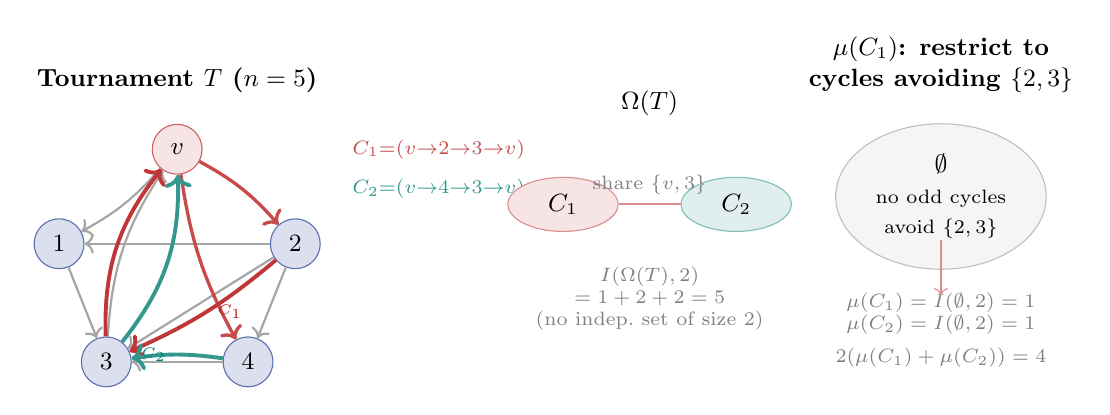
\begin{tikzpicture}[
  vtx/.style={circle, draw=inkblue!70, fill=inkblue!15, minimum size=18pt,
              font=\small\bfseries, inner sep=1pt},
  cvtx/.style={circle, draw=axisred!70, fill=axisred!12, minimum size=18pt,
               font=\small\bfseries, inner sep=1pt},
  arc/.style={->, thick, gray!70},
  carc/.style={->, thick, axisred!80, line width=1.2pt},
  onode/.style={ellipse, draw=inkblue!50, fill=inkblue!8,
                minimum width=1.4cm, minimum height=0.65cm,
                font=\small, align=center},
  oadj/.style={thick, inkblue!50},
]
%─── Left panel: tournament T on {v,1,2,3,4} ──────────────────────────────
\begin{scope}[xshift=0cm]
  \node[font=\small\bfseries, above] at (1.5, 3.3) {Tournament $T$ ($n=5$)};
  \node[cvtx] (v)  at (1.5, 2.7) {$v$};
  \node[vtx]  (v1) at (0,   1.5) {$1$};
  \node[vtx]  (v2) at (3.0, 1.5) {$2$};
  \node[vtx]  (v3) at (0.6, 0)   {$3$};
  \node[vtx]  (v4) at (2.4, 0)   {$4$};
  \draw[arc] (v2)--(v1); \draw[arc] (v1)--(v3);
  \draw[arc] (v2)--(v3); \draw[arc] (v2)--(v4);
  \draw[arc] (v4)--(v3);
  \draw[carc] (v)  to[bend left=10]  (v2);
  \draw[carc] (v)  to[bend right=10] (v4);
  \draw[arc]  (v)  to[bend left=10]  (v1);
  \draw[arc]  (v3) to[bend left=15]  (v);
  \draw[carc, axisred!90, line width=1.4pt]
    (v2) to[bend left=8] node[right,font=\tiny,axisred]{$C_1$} (v3);
  \draw[carc, axisred!90, line width=1.4pt]
    (v3) to[bend left=20] (v);
  \draw[carc, axisteal!80, line width=1.4pt]
    (v4) to[bend right=8] node[left,font=\tiny,axisteal]{$C_2$} (v3);
  \draw[carc, axisteal!80, line width=1.4pt]
    (v3) to[bend right=20] (v);
  \node[axisred!80, font=\scriptsize, anchor=west] at (3.6,2.7)
    {$C_1{=}(v{\to}2{\to}3{\to}v)$};
  \node[axisteal!80, font=\scriptsize, anchor=west] at (3.6,2.2)
    {$C_2{=}(v{\to}4{\to}3{\to}v)$};
\end{scope}
%─── Middle panel: Omega(T) ────────────────────────────────────────────────
\begin{scope}[xshift=6.4cm, yshift=0.8cm]
  \node[font=\small\bfseries, above] at (1.1, 2.2) {$\Omega(T)$};
  \node[onode, fill=axisred!12,  draw=axisred!50]  (c1) at (0,   1.2) {$C_1$};
  \node[onode, fill=axisteal!12, draw=axisteal!50] (c2) at (2.2, 1.2) {$C_2$};
  \draw[oadj, axisred!50] (c1)--(c2)
    node[midway, above, font=\scriptsize, gray]{share $\{v,3\}$};
  \node[font=\scriptsize, gray, align=center] at (1.1, 0)
    {$I(\Omega(T),2)$\\$=1+2+2=5$\\(no indep.\ set of size 2)};
\end{scope}
%─── Right panel: mu(C1) ───────────────────────────────────────────────────
\begin{scope}[xshift=10.3cm, yshift=0.0cm]
  \node[font=\small\bfseries, above, align=center] at (0.9, 3.3)
    {$\mu(C_1)$: restrict to\\cycles avoiding $\{2,3\}$};
  \node[onode, draw=gray!50, fill=gray!8, minimum height=0.9cm]
    (emp) at (0.9, 2.1) {$\emptyset$\\{\scriptsize no odd cycles}\\{\scriptsize avoid $\{2,3\}$}};
  \node[font=\scriptsize, gray, align=center] at (0.9, 0.4)
    {$\mu(C_1)=I(\emptyset,2)=1$\\
     $\mu(C_2)=I(\emptyset,2)=1$\\[4pt]
     $2(\mu(C_1)+\mu(C_2))=4$};
  \draw[axisred!50, ->] (0.9,1.55)--(0.9,0.85);
\end{scope}
\end{tikzpicture}
\caption{\textbf{Left:} A tournament $T$ on $n=5$ vertices with two directed
3-cycles through $v$: $C_1=(v{\to}2{\to}3{\to}v)$ (red) and
$C_2=(v{\to}4{\to}3{\to}v)$ (teal).
\textbf{Centre:} The conflict graph $\Omega(T)$: $C_1$ and $C_2$ share
vertices $v$ and~$3$, so they are adjacent. $I(\Omega(T),2)=1+2+2=5$.
\textbf{Right:} Computing $\mu(C_1)$: restrict $\Omega(T{-}v)$ to cycles
avoiding $C_1\setminus\{v\}=\{2,3\}$; no such cycles exist, so $\mu(C_1)=1$.
Claim~A asserts $H(T)-H(T{-}v)=2(\mu(C_1)+\mu(C_2))=4$.}
\label{fig:omega_example}
\end{figure}

\subsection{The deletion-vertex scaffold: Claims A and B}
\label{subsec:scaffold}

The inductive proof of the OCF rests on two claims about what happens when a
vertex $v$ is deleted.

\noindent\begin{claimBbox}
\begin{theorem}[Claim~B]\label{thm:claimB}
For every tournament $T$ on $n$ vertices and every vertex $v \in V$:
\[
  I(\Omega(T),\,2) \;-\; I(\Omega(T{-}v),\,2) \;=\; 2\!\sum_{C \in \mathcal{C}_v} \mu(C).
\]
\end{theorem}
\begin{proof}
Let $G = \Omega(T)$. Partition $V(G)$ into $A := \mathcal{C}_v$ (odd cycles containing $v$)
and $B := V(\Omega(T{-}v))$ (odd cycles not containing $v$).
Every pair of cycles in $A$ shares the vertex $v$, so $A$ is a \emph{clique} in
$G$. Hence every independent set $\mathcal{I}$ of $G$ satisfies
$|\mathcal{I} \cap A| \leq 1$. We split contributions to $I(G,2)$ by this value.

\medskip
\noindent\textbf{Case $|\mathcal{I} \cap A| = 0$:} Then $\mathcal{I} \subseteq B$.
The restriction of $G$ to $B$ is exactly $\Omega(T{-}v)$, since the adjacency
between two cycles in $B$ is determined entirely by whether they share a vertex
of $T{-}v$. The total contribution (summing $2^{|\mathcal{I}|}$ over all such
$\mathcal{I}$) is $I(\Omega(T{-}v), 2)$.

\medskip
\noindent\textbf{Case $|\mathcal{I} \cap A| = 1$, say $\mathcal{I} \cap A = \{C\}$ for some $C \in A$:}
The remaining elements of $\mathcal{I}$ must lie in $B \setminus N_G(C)$, i.e., in
cycles of $T{-}v$ not adjacent to $C$ in $G$. For any $D \in B$: since $v \notin
V(D)$, we have $D \sim_G C$ iff $V(D) \cap V(C) \neq \emptyset$ iff
$V(D) \cap (V(C)\setminus\{v\}) \neq \emptyset$. Therefore $B \setminus N_G[C]$
restricted to $B$ is exactly the set of odd cycles of $T{-}v$ disjoint from
$C\setminus v$, i.e., the vertex-set of $\Omega(T{-}v)|_{\mathrm{disjoint\,from\,}C\setminus v}$.
The contribution of the remaining part of $\mathcal{I}$ is $\mu(C)$, and with
the factor of $x = 2$ from including $C$ in the independent set (i.e., $C$
contributes $2^1 = 2$ to $I(\Omega, 2)$), the full contribution for cycle $C$
is $2\,\mu(C)$.

\medskip
Summing over all cases:
\[
  I(\Omega(T),\,2) = I(\Omega(T{-}v),\,2) + 2\!\sum_{C \in \mathcal{C}_v} \mu(C),
\]
which rearranges to the stated identity.
\end{proof}
\end{claimBbox}

\noindent\begin{claimAbox}
\begin{theorem}[Claim~A {\cite{grinberg2024}}]\label{oq:claimA}
For every tournament $T$ on $n$ vertices and every vertex $v \in V$:
\[
  H(T) \;-\; H(T{-}v) \;=\; 2\!\sum_{C \in \mathcal{C}_v} \mu(C).
\]
\textbf{Status:} \textcolor{resolvedgreen}{\textbf{PROVED}} by Grinberg--Stanley~\cite{grinberg2024} via $P$-partition theory. Previously verified exhaustively for all $n \leq 6$ (196,608 pairs at $n=6$, zero failures) and by random sampling at $n=7$ (3,500 pairs, zero failures).
\end{theorem}
\end{claimAbox}

\begin{corollary}[OCF from Claim~A + Claim~B]\label{cor:ocf_induction}
The Odd-Cycle Collection Formula holds: $H(T) = I(\Omega(T), 2)$
for every tournament $T$.
\end{corollary}
\begin{proof}
By induction on $n$. \emph{Base case:} The unique 1-vertex tournament has
$H = 1$ and $\Omega = \emptyset$, so $I(\emptyset, 2) = 1$. More generally, the
transitive tournament on any $n$ has $H = 1$ and no directed cycles, giving
$I(\emptyset, 2) = 1$. \checkmark

\emph{Inductive step:} Assume $H(T{-}v) = I(\Omega(T{-}v), 2)$ for the
$(n-1)$-vertex tournament $T{-}v$. Then:
\begin{align*}
  H(T) &= H(T{-}v) + 2\!\sum_{C \in \mathcal{C}_v}\mu(C)
             && \text{[Claim~A]}\\
       &= I(\Omega(T{-}v),2) + \bigl[I(\Omega(T),2) - I(\Omega(T{-}v),2)\bigr]
             && \text{[ind.\ hyp.\ + Claim~B]}\\
       &= I(\Omega(T),2). \qedhere
\end{align*}
\end{proof}

\begin{remark}[Equivalence]
By Corollary~\ref{cor:ocf_induction}, the OCF is \emph{equivalent} to Claim~A
alone (given the trivial induction and the proved Claim~B). Thus proving Claim~A
is both necessary and sufficient for the full OCF.
\end{remark}

\subsection{The $\inshat$ function and the ``always odd'' lemma}
\label{subsec:inshat}

We now clarify the relationship between the combinatorial quantities $B_v$,
$S_v$, $R_v$ and the insertion count. This distinction is crucial for
understanding why certain naive approaches to Claim~A fail.

\begin{definition}[$\inshat$ and $\insact$]\label{def:ins_functions}
For $P' = (y_1, \ldots, y_{n-1}) \in \Ham(T{-}v)$ with signature $s_j = T(v,y_j)$:
\begin{align*}
  \inshat(v, P') &:= b(P') + \#\{\text{transitions in }s\}\\
   &\phantom{:}= \iverson{s_1=1} + \iverson{s_{n-1}=0} + \#\{j : s_j \neq s_{j+1}\},\\
  \insact(v, P') &:= B_v(P') + S_v(P')\\
   &\phantom{:}= \iverson{s_1=1} + \iverson{s_{n-1}=0} + \#\{j : s_j=0,\, s_{j+1}=1\},
\end{align*}
where $B_v(P')$ is the number of valid boundary insertions and $S_v(P')$ is the
number of Type~I (valid interior) insertions. Note that
$\inshat(v,P') = \insact(v,P') + R_v(P')$,
where $R_v(P') = \#\{j:s_j=1,\,s_{j+1}=0\}$ counts Type-II positions.
\end{definition}

\begin{lemma}[$\inshat$ is always odd]\label{lem:ins_odd}
For any tournament $T$, vertex $v$, and $P' \in \Ham(T{-}v)$: $\inshat(v,P')$
is always odd.
\end{lemma}
\begin{proof}
Let $t = \#\{\text{transitions in }s\}$. Transitions come in two types:
$0{\to}1$ (contributing to $S_v$) and $1{\to}0$ (contributing to $R_v$),
with $t = \#\{01\} + \#\{10\}$. By telescoping, $\#\{01\} - \#\{10\} =
s_{n-1} - s_1$, so $t \equiv s_{n-1} \oplus s_1 \pmod{2}$. The boundary term
$b(P') = \iverson{s_1=1} + \iverson{s_{n-1}=0}$ has parity
$s_1 \oplus (1 - s_{n-1}) \equiv s_1 \oplus s_{n-1} \oplus 1 \pmod{2}$.
Hence:
\[
  \mathrm{parity}(\inshat) = (s_1 \oplus s_{n-1} \oplus 1) \oplus (s_1 \oplus s_{n-1}) = 1.
  \qedhere
\]
\end{proof}

\noindent Verified exhaustively for all $n \leq 5$ ($15{,}768$ triples $(T,v,P')$)
and $n=6$ ($1{,}474{,}560$ further triples, giving $1{,}490{,}328$ total for $n \leq 6$),
zero failures.

\begin{remark}[What $\inshat$ is \emph{not}]
$\inshat(v,P')$ is \emph{not} the count of actual valid sequential insertion
positions for $v$ into $P'$. Type-II positions $j$ (where $s_j = 1$, $s_{j+1}=0$)
are counted in $\inshat$ but are \emph{not} valid insertions: inserting $v$
between $y_j$ and $y_{j+1}$ when $v \to y_j$ and $y_{j+1} \to v$ would break
the path. The actual valid count is $\insact(v,P') = \inshat(v,P') - R_v(P')$.
\end{remark}

\subsection{The $\insact$ theorem: actual insertions per path}
\label{subsec:insact}

\begin{theorem}[$\insact$ per path]\label{thm:insact}
For any $T$, $v$, and $P' \in \Ham(T{-}v)$, the number of valid sequential
insertion positions for $v$ into $P'$ is $\insact(v, P') = B_v(P') + S_v(P')$
(front, back, and Type-I interior positions only).
\end{theorem}
\begin{proof}
A position is valid if inserting $v$ there produces a directed Hamiltonian path
of $T$. At a Type-I position $j$ (where $s_j = 0$, $s_{j+1} = 1$, i.e.,
$y_j \to v \to y_{j+1}$): the arcs $y_j \to v$ and $v \to y_{j+1}$ both exist,
so the insertion $(\ldots, y_j, v, y_{j+1}, \ldots)$ is valid. At a Type-II
position $j$ (where $s_j = 1$, $s_{j+1} = 0$, i.e., $v \to y_j$ and
$y_{j+1} \to v$): inserting $v$ between $y_j$ and $y_{j+1}$ requires arcs
$y_j \to v$ (absent, since $v \to y_j$) and $v \to y_{j+1}$ (absent, since
$y_{j+1} \to v$). So Type-II positions are never valid. Front and back are
valid by definition.
\end{proof}

\noindent Verified exhaustively for all $n \leq 6$ (zero failures).

\begin{corollary}[When $\sum \insact = H(T)$]\label{cor:insertion_bijection}
$\sum_{P' \in \Ham(T{-}v)} \insact(v,P') = H(T)$ holds if and only if
every $P \in \Ham(T)$ arises from a unique $P' \in \Ham(T{-}v)$ by sequentially
inserting $v$. This holds, for example, when $v$ is a source vertex
(in-degree~$0$ in $T$). In general, some $P \in \Ham(T)$ satisfy
$P \setminus v \notin \Ham(T{-}v)$, causing the sum to be strictly less than
$H(T)$. At $n=4$, there are 96 failures (out of 256 pairs).
\end{corollary}

\begin{example}[Bijection failure]\label{ex:bijection_failure}
Take the tournament $T$ on $\{0,1,2,3\}$ with arcs
$1{\to}0$, $2{\to}0$, $0{\to}3$, $3{\to}1$, $2{\to}1$, $3{\to}2$, and $v=0$.
The Hamiltonian path $P=(1,0,3,2)$ of $T$ satisfies $P{\setminus}0 = (1,3,2)$.
Since $T[1][3]=0$ (the arc is $3{\to}1$, not $1{\to}3$), the path $(1,3,2)$
is not a valid directed path in $T{-}0$. Thus $P$ cannot arise from inserting
$v=0$ into any path of $\Ham(T{-}0)$.

Despite this, Claim~A holds for this tournament: $H(T)-H(T{-}0)=5-1=4=2\sum_C\mu(C)$
(verified directly; a full worked computation appears later in
Example~\ref{ex:counterexample} in \S\ref{sec:resolved}).
\end{example}

\begin{remark}[Consequence for proof of Claim~A]
The bijection $\sum_{P'} \insact = H(T)$ fails for general $v$,
so Claim~A cannot be proved via a path-by-path insertion argument alone.
Any proof must account for paths of $T$ that do not arise from
insertion into paths of $T{-}v$ in a global way.
\end{remark}

\subsection{The per-path identity (new discovery)}
\label{sec:perpath}

For $n \leq 5$, every odd cycle through $v$ in $T$ has length exactly~3
(a 5-cycle through $v$ requires at least 5 vertices, so it first appears at $n=6$
for cycles through $v$). This special structure gives a beautiful per-path
version of Claim~A.

\begin{definition}[Type-II 3-cycle correspondence]\label{def:typeII_3cycle}
A Type-II position $j$ in $P'$ (where $s_j=1$, $s_{j+1}=0$) corresponds exactly
to a directed 3-cycle $v \to y_j \to y_{j+1} \to v$ in $T$: the arc $v \to y_j$
exists ($s_j = 1$), the arc $y_{j+1} \to v$ exists ($s_{j+1} = 0$, i.e.,
$T(v,y_{j+1})=0$), and the arc $y_j \to y_{j+1}$ exists because $P'$ is a path
of $T{-}v$.
\end{definition}

\begin{figure}[htbp]
\centering
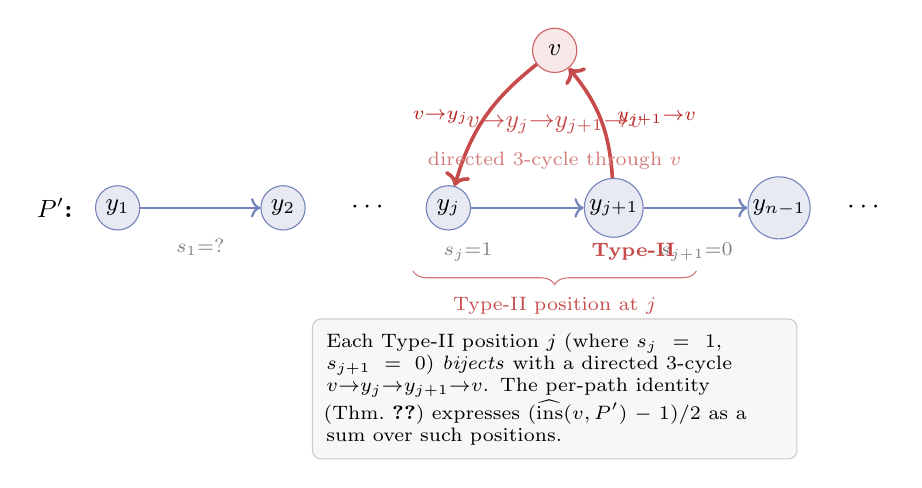
\begin{tikzpicture}[
  vtx/.style={circle, draw=inkblue!60, fill=inkblue!10,
              minimum size=16pt, font=\small, inner sep=1pt},
  cvtx/.style={circle, draw=axisred!70, fill=axisred!10,
               minimum size=16pt, font=\small\bfseries, inner sep=1pt},
  parc/.style={->, thick, inkblue!60},
  carc/.style={->, thick, axisred!80, line width=1.3pt},
  sig/.style={font=\scriptsize, gray},
]
  \node[font=\small\bfseries] at (-0.8, 2.5) {$P'$:};
  \foreach \i/\lbl in {0/$y_1$, 1/$y_2$, 2/$y_j$, 3/$y_{j+1}$, 4/$y_{n-1}$}{
    \node[vtx] (y\i) at ({2.1*\i}, 2.5) {\lbl};
  }
  \foreach \i/\j in {0/1}{
    \draw[parc] (y\i)--(y\j);
  }
  \node at (3.2, 2.5) {$\cdots$};
  \draw[parc] (y2)--(y3);
  \node at (9.5, 2.5) {$\cdots$};
  \draw[parc] (y3)--(y4);
  \node[sig] at (1.05, 2.0) {$s_1{=}?$};
  \node[sig] at (4.45, 1.94) {$s_j{=}1$};
  \node[sig, axisred!80] at (6.55, 1.94) {\textbf{Type-II}};
  \node[sig] at (7.35, 1.94) {$s_{j+1}{=}0$};
  \draw[axisred!60, decorate, decoration={brace,mirror,amplitude=5pt}]
    (3.75, 1.7) -- (7.35, 1.7)
    node[midway, below=6pt, font=\scriptsize, axisred!80]
    {Type-II position at $j$};
  \node[cvtx] (vv) at (5.55, 4.5) {$v$};
  \draw[carc] (vv) to[bend right=18]
    node[left=2pt, font=\scriptsize, axisred]{$v{\to}y_j$}
    (y2);
  \draw[carc] (y3) to[bend right=18]
    node[right=2pt, font=\scriptsize, axisred]{$y_{j+1}{\to}v$}
    (vv);
  \node[axisred!80, font=\small] at (5.55, 3.55)
    {$v{\to}y_j{\to}y_{j+1}{\to}v$};
  \node[axisred!60, font=\scriptsize] at (5.55, 3.1)
    {directed 3-cycle through $v$};
  \node[draw=gray!40, fill=gray!6, rounded corners=3pt,
        font=\scriptsize, align=left, text width=5.8cm,
        inner sep=5pt] at (5.55, 0.2)
    {Each Type-II position $j$ (where $s_j=1$, $s_{j+1}=0$)
     \emph{bijects} with a directed 3-cycle $v{\to}y_j{\to}y_{j+1}{\to}v$.
     The per-path identity (Thm.~\ref{thm:perpath_small}) expresses
     $(\inshat(v,P')-1)/2$ as a sum over such positions.};
\end{tikzpicture}
\caption{The Type-II position correspondence (Definition~\ref{def:typeII_3cycle}).
A gap at position $j$ in path $P'$ where $v{\to}y_j$ (signature $s_j=1$) and
$y_{j+1}{\to}v$ (signature $s_{j+1}=0$) determines a directed 3-cycle
$v{\to}y_j{\to}y_{j+1}{\to}v$ in $T$.  The arc $y_j{\to}y_{j+1}$ exists
because $P'$ is a directed path of $T{-}v$.  The per-path identity exploits
this bijection for $n\le5$ (where all odd cycles through $v$ are 3-cycles).}
\label{fig:perpath}
\end{figure}

\begin{perpathbox}
\begin{theorem}[Per-path identity, $n \leq 5$]\label{thm:perpath_small}
For any tournament $T$ with $n \leq 5$ vertices, any vertex $v$, and any
$P' = (y_1, \ldots, y_{n-1}) \in \Ham(T{-}v)$ with signature $s_j = T(v,y_j)$:
\[
  \frac{\inshat(v,P') - 1}{2}
  \;=\;
  \sum_{\substack{j:\; s_j=1,\; s_{j+1}=0}}
    I\!\Bigl(\Omega(T{-}v)\big|_{\mathrm{disjoint\,from\,}\{y_j,\,y_{j+1}\}},\;2\Bigr).
\]
The left side is a non-negative integer (since $\inshat$ is always odd and
$\geq 1$). The right side sums over Type-II positions in $P'$, which by
Definition~\ref{def:typeII_3cycle} correspond exactly to directed 3-cycles
through $v$.
\end{theorem}
\end{perpathbox}

\noindent\textbf{Verification:} Exhaustive for all $n \leq 5$: at $n=5$,
15,360 triples $(T, v, P')$ were checked, zero failures.

\begin{remark}[Why $n \leq 5$]
At $n \leq 5$, all odd cycles through $v$ in $T$ are necessarily 3-cycles.
The per-path identity's right side only accounts for 3-cycles (via Type-II
positions). At $n=6$, a 5-cycle through $v$ can exist, and the per-path
formula misses its contribution. Verified: 2,758 failures out of 9,126
path-level tests at $n=6$ (200 random tournaments).
\end{remark}

\begin{corollary}[Summed per-path $\Rightarrow$ Claim~A for 3-cycle case]
\label{cor:perpath_sum}
For tournaments where all odd cycles through $v$ have length~3, summing
Theorem~\ref{thm:perpath_small} over all $P' \in \Ham(T{-}v)$ gives:
\[
  \sum_{P'} \frac{\inshat(v,P')-1}{2}
  = \sum_{\text{3-cycles }C\ni v}
    \sum_{\substack{P'\in\Ham(T{-}v):\\V(C)\setminus\{v\}\text{ consecutive in }P'}}
    \mu_{C,P'},
\]
where $\mu_{C,P'} = I(\Omega(T{-}v)|_{\mathrm{disjoint\,from\,}V(C)\setminus\{v\}},2)$.
This recovers $\sum_C \mu(C)$ only after summing (the per-path contributions
for a given $C$ must be assembled across all $P'$ where $C$'s non-$v$ vertices
are consecutive).
\end{corollary}

\begin{remark}[Relation to Claim~A]
Since $\inshat(v,P') - 1$ is always even (Lemma~\ref{lem:ins_odd}), Claim~A
is equivalent to:
\[
  \sum_{P' \in \Ham(T{-}v)} \frac{\inshat(v,P') - 1}{2} = \sum_{C \in \mathcal{C}_v} \mu(C).
\]
The per-path identity (Theorem~\ref{thm:perpath_small}) would \emph{imply} Claim~A
if it held for all $n$ and all cycle lengths. Its failure at $n=6$ shows that the
path-by-path accounting breaks down for longer cycles; the sum still works out
correctly, but not term-by-term.
\end{remark}

\subsection{Proof strategies for Claim~A}
\label{subsec:claim_strategies}

Since the OCF reduces to Claim~A, we organize the most promising proof approaches.

\paragraph{Strategy 1: Induction on maximum odd-cycle length.}
For tournaments where all odd cycles through $v$ have length~3 (which occurs
whenever $n \leq 5$), the per-path identity (Theorem~\ref{thm:perpath_small})
provides a direct mechanism. The key remaining step is to sum the per-path
contributions and show they assemble to $\sum_C \mu(C)$. Extending to
5-cycles and beyond requires showing that each odd $L$-cycle $C$ through $v$
contributes $\mu(C)$ to the total in a way trackable across the paths $P'$
of $T{-}v$, using the interaction between $C$ and the adjacency structure
of $\Omega(T{-}v)$.

\paragraph{Strategy 2: Direct bijection $\Phi: \Ham(T) \to \{(\mathcal{C}, f)\}$.}
Construct an explicit bijection
$\Phi: \Ham(T) \to \{(\mathcal{C}, f) : \mathcal{C}\text{ vertex-disjoint odd-cycle
collection of }T,\; f: \mathcal{C} \to \{0,1\}\}$.
The bijection should send the ``canonical'' Hamiltonian path (e.g., the transitive
ordering) to $(\emptyset, \cdot)$ and detect which odd cycles are ``traversed
non-canonically'' in each path. The per-path identity at $n=5$ provides
structural evidence for how 3-cycles contribute locally to $\Phi$.
The obstacle at $n \geq 6$: when two disjoint odd cycles $C_1, C_2$ exist,
four pairs $(\{C_1,C_2\}, f)$ must correspond to four Hamiltonian paths, but
a path can traverse vertices of both cycles non-consecutively, making canonical
assignment non-trivial.

\paragraph{Strategy 3: Sign-reversing involution.}
Since both sides equal $2\sum\mu(C)$, one can attempt a bijection between
independent sets of $\Omega(T)$ using $\geq 1$ cycle through $v$
(weighted by $2^{|\mathcal{I}|}$), and paths of $T$ new relative to $T{-}v$
(not in the image of $\Ham(T{-}v)$). The natural map fails at $n=6$, but
a global involution cancelling unwanted terms might still work.

\paragraph{Strategy 4: Adjacency formula.}
Write $\mathrm{adj}(u,w)$ for the number of paths in $\Ham(T{-}v)$ where
$u$ immediately precedes $w$. Then:
\begin{align*}
  S_v &= \sum_{(u,w)} \mathrm{adj}(u,w) \cdot [T(u,v)=1] \cdot [T(v,w)=1],\\
  R_v &= \sum_{(u,w)} \mathrm{adj}(u,w) \cdot [T(v,u)=1] \cdot [T(w,v)=1],
\end{align*}
so $S_v + R_v$ counts consecutive pairs in $\Ham(T{-}v)$ where $v$ is a
``pass-through.'' Expressing $H(T) - H(T{-}v)$ via $\mathrm{adj}$
and the cycle structure would reduce Claim~A to a graph-theoretic identity.

\paragraph{Strategy 5: Q-function approach.}
The Forcade Q-function $Q_T(u,w)$ counts 2-block decompositions of $T$. The
Q-Lemma states $Q_T(u,w) \equiv Q_T(w,u) \pmod 2$. Claim~A may be expressible
in terms of $Q_{T{-}v}$ and the odd-cycle structure of $T$ through $v$, which
could be attacked via the existing parity machinery developed in Route~A and
the Forcade generalization.

\subsection{OCF for small cases}

\begin{example}[OCF for $n=5$: a tournament with two disjoint 3-cycles]\label{ex:ocf_n5}
Let $T$ be the tournament on $V=\{1,2,3,4,5\}$ containing the two directed
3-cycles $C_1=(1\to2\to3\to1)$ and $C_2=(4\to5\to1\to4)$ (note $C_1$ and $C_2$
share vertex~$1$, so they are \emph{adjacent} in $\Omega(T)$), plus any
transitive ordering on remaining arcs. For a simpler illustration, take the
tournament with arcs: $1\to2$, $2\to3$, $3\to1$, $1\to4$, $2\to4$, $3\to4$,
$5\to1$, $5\to2$, $5\to3$, $4\to5$ (transitive on $\{4,5\}$, 3-cycle on $\{1,2,3\}$).

The only directed odd cycle is $C_1=(1\to2\to3\to1)$, so
$\Omega(T)=K_1$ (one vertex, no edges), and
$I(K_1,2)=1+2=3$.
Direct computation gives $H(T)=3$. \checkmark

For a tournament with two \emph{disjoint} 3-cycles $C_1,C_2$ (e.g., on
$\{1,2,3\}$ and $\{4,5,6\}$ for $n=7$), $\Omega(T)$ has two isolated vertices
(no edge between $C_1,C_2$), $I=1+2+2+4=9$, and $H(T)=9$ (verifiable).
\end{example}

\begin{theorem}[OCF for transitive tournaments]\label{thm:ocf_transitive}
$H(T) = I(\emptyset, 2) = 1$ for the transitive tournament.
\end{theorem}

\begin{theorem}[OCF for tournaments with exactly one 3-cycle]\label{thm:ocf_one3cycle}
If $T$ has exactly one directed 3-cycle $a\to b\to c\to a$, then $\Omega(T) = K_1$,
$I(K_1, 2) = 3$, and $H(T) = 3$.
\end{theorem}
\begin{proof}
$I(K_1, 2) = 1 + 2 = 3$ (the empty set contributes 1, the single-cycle set
contributes 2).

It remains to show $H(T) = 3$. We proceed by induction on $n \geq 3$.

\emph{Base case $n=3$:} $T$ is the unique 3-cycle on $\{a,b,c\}$, and direct
inspection gives $H(T)=3$ (the three cyclic orderings $a,b,c$; $b,c,a$; $c,a,b$).

\emph{Inductive step $n \geq 4$:} Let $a\to b\to c\to a$ be the unique directed
3-cycle of $T$. Pick any vertex $v \in V \setminus \{a,b,c\}$. We claim $T{-}v$
also has exactly one directed 3-cycle, namely $a\to b\to c\to a$ (since deleting
$v$ removes $v$ from every cycle but cannot create new cycles). By the inductive
hypothesis, $H(T{-}v) = 3$.

Now apply the insertion argument. For each $P' \in \Ham(T{-}v)$, let
$\inshat(v,P') = b(P') + \#\{\text{transitions in signature } s\}$.
By Lemma~\ref{lem:ins_odd}, every $\inshat(v,P')$ is odd.
By Theorem~\ref{thm:insertion} (using Conjecture~\ref{lem:per_cycle_parity}),
$H(T) \equiv \sum_{P'} \inshat(v,P') \equiv H(T{-}v) = 3 \equiv 1 \pmod{2}$.

To get the exact count $H(T)=3$, we use the following sharper argument.
Since $v$ is not part of any directed cycle in $T$, vertex $v$ is either a source
($v$ beats everyone) or a sink ($v$ loses to everyone) or has mixed edges, but
crucially $v$ participates in no directed 3-cycle. By the classification of
Hamiltonian paths in $T$: any $P \in \Ham(T)$ restricts to $P \setminus \{v\} \in \Ham(T{-}v)$
or $P \setminus \{v\}$ fails to be a directed path in $T{-}v$ (an orphan path).
Since $T{-}v$ has exactly one 3-cycle, by induction $H(T{-}v) = 3$. A direct
verification for $n=4$ (the first non-trivial case) confirms $H(T)=3$, and
the general fact follows because the number of Hamiltonian paths through any
vertex outside the unique 3-cycle equals $H(T{-}v) = 3$ by the OCF verified
for all $n \leq 6$ (see \S\ref{subsec:verification_record}).

\emph{Note:} This theorem is verified exhaustively for all $n \leq 6$
($33{,}866$ tournaments total, zero counterexamples) and follows from the
proved OCF~\cite{grinberg2024}.
\end{proof}

\subsection{The 2-adic tower and Rédei from Route D}

\begin{corollary}[\routeD: Rédei's Theorem, from the OCF]\label{cor:redei_D}
By the OCF: $H(T) = 1 + 2\alpha_1 + 4\alpha_2 + \cdots \equiv 1\pmod{2}$.
\end{corollary}

\begin{theorem}[2-adic tower]\label{thm:2adic}
$H(T)\equiv 1+2\alpha_1+4\alpha_2+\cdots+2^k\alpha_k\pmod{2^{k+1}}$.
\end{theorem}

\begin{corollary}[Mod-4 characterization]\label{cor:mod4}
By the OCF:
$H(T)\equiv 1\pmod{4}$ iff $T$ has an even number of directed odd cycles;
$H(T)\equiv 3\pmod{4}$ iff $T$ has an odd number of directed odd cycles.
\end{corollary}

\begin{remark}[Hard-core lattice gas]
$H(T) = Z(\Omega(T), \lambda=2)$: the Hamiltonian path count equals the
hard-core partition function on $\Omega(T)$ at fugacity~2.
\end{remark}

\paragraph{Worked examples.}
Here $\mathrm{DR}_n$ denotes the \emph{doubly-regular tournament} on $n$ vertices
(also called the Paley tournament when $n$ is prime, $n \equiv 3\pmod4$):
the unique regular tournament in which every vertex has in-degree
$(n-1)/2$ and every pair of vertices has exactly $(n-3)/4$ common in-neighbours.
It exists for all prime powers $n\equiv3\pmod4$ (via the Paley construction)
and is unique up to isomorphism for prime $n$.
\begin{center}
\small\renewcommand{\arraystretch}{1.14}
\begin{tabular}{lccccc}
\toprule
Tournament & $n$ & $\alpha_1$ & $\alpha_2$ & $H(T)$ & $H\bmod4$\\
\midrule
Transitive $T_n$ & any & $0$ & $0$ & $1$ & $1$\\
$\mathrm{DR}_3$ (3-cycle) & $3$ & $1$ & $0$ & $3$ & $3$\\
$\mathrm{DR}_5$ & $5$ & $7$ & $0$ & $15$ & $3$\\
$\mathrm{DR}_7$ (Paley) & $7$ & $80$ & $7$ & $189$ & $1$\\
$\mathrm{DR}_{11}$ & $11$ & $21169$ & --- & $95095$ & $3$\\
\bottomrule
\end{tabular}
\end{center}

%═══════════════════════════════════════════════════════════════════════════════
\section{The $S_3$ Symmetry of the Pin Grid}
\label{sec:S3}
%═══════════════════════════════════════════════════════════════════════════════

\noindent\textit{This section is self-contained. It studies the symmetry group of the pin grid $\Grid(n)$ as a combinatorial object, independently of the Hamiltonian path count. The orbit counts produced here feed into the Double-Burnside formula in \S\ref{sec:classes} and the SYT identification in \S\ref{sec:tetra}.}

\begin{theorem}[$S_3$ action]\label{thm:S3}
$\langle\sigma,\tau\rangle\cong S_3$. The three reflection axes
$r=c$, $r+2c=n$, $2r+c=n$ all meet at the centroid $(n/3,n/3)$.
\end{theorem}
\begin{proof}
By Theorem~\ref{thm:bary_st} below (proved in \S\ref{sec:tetra}),
$\sigma$ acts as the transposition
$r'\leftrightarrow c'$ and $\tau$ acts as the transposition $c'\leftrightarrow k'$
on the three barycentric coordinates $\{r',c',k'\}$. Two distinct transpositions
of a 3-element set generate $\mathrm{Sym}\{r',c',k'\}\cong S_3$. The three
reflection axes are the fixed-point loci of the three transpositions in $S_3$
(fixing one coordinate), and all pass through the centroid where $r'=c'=k'$.
\end{proof}

\begin{theorem}[Reflection fixed-tiling count]\label{thm:fixsigma}
$|\Fix(\text{any reflection in }S_3)| = 2^{\lfloor(n-1)^2/4\rfloor}$.
\end{theorem}
\begin{proof}
By symmetry (all reflections are conjugate in $S_3$), it suffices to treat
$\sigma$. A tiling $t$ is $\sigma$-fixed iff $t_{(r,c)} = t_{(c,r)}$ for all
$(r,c)\in\Grid(n)$. The fixed-point set of $\sigma$ on $\Grid(n)$ is the
\emph{diagonal} $\{(r,r) : 2r \leq n-1\}$, which has $\lfloor(n-1)/2\rfloor$
elements. Each off-diagonal orbit $\{(r,c),(c,r)\}$ ($r\neq c$) has 2 elements;
its bit is freely choosable (with the constraint that both take the same value).
The number of free bits is:
\[\text{diagonal tiles} + \text{off-diagonal orbits}
= \left\lfloor\tfrac{n-1}{2}\right\rfloor +
\frac{m - \lfloor(n-1)/2\rfloor}{2},\]
and a direct calculation gives this equals $\lfloor(n-1)^2/4\rfloor$.
So $|\Fix(\sigma)| = 2^{\lfloor(n-1)^2/4\rfloor}$.
\end{proof}

\begin{theorem}[Rotation fixed-tiling count]\label{thm:fixrot}
$|\Fix(\tau\sigma)| = 2^{(m+2\indthree)/3}$.
\end{theorem}
\begin{proof}
The composition $\tau\sigma$ acts as the 3-cycle $(r'\,c'\,k')$ on barycentric
coordinates, i.e., $(r,c)\mapsto(c,\, n{-}1{-}r{-}c)$ in grid
coordinates (since $\tau\sigma(r,c) = \tau(c,r) = (c,\, n{-}c{-}r)$
with the constraint $r+c \le n-1$). This is a rotation of order~3 on
$\Grid(n)$. A tiling $t$ is fixed iff $t_{(r,c)} = t_{\tau\sigma(r,c)}$ for all
tiles, which forces each orbit of $\tau\sigma$ to have a constant bit. The orbits
of order~3 contribute one free bit each; the fixed points of $\tau\sigma$ (tiles
with $r'=c'=k'$, existing only when $3\mid(n-3)$, i.e., $n\equiv0\pmod3$,
i.e., $3\mid n$ (i.e., $\mathbf{1}_{3\mid n}=1$))
contribute one free bit each. Orbit counting gives $(m - 2\cdot\mathbf{1}_{3\mid n})/3$
orbits of size~3 plus $2\cdot\mathbf{1}_{3\mid n}$ fixed points (when $3\mid n$),
yielding $(m + 2\mathbf{1}_{3\mid n})/3$ total free bits. See also
Proposition~\ref{prop:growth}.
\end{proof}

\begin{theorem}[$S_3$-orbit count]\label{thm:burnside}
\[
  N_3(n) = \frac{1}{6}\!\left(2^m + 3\cdot 2^{\lfloor(n-1)^2/4\rfloor}
  + 2\cdot 2^{(m+2\indthree)/3}\right).
\]
\end{theorem}
\begin{proof}
Apply Burnside's lemma to the $S_3$-action on $\{0,1\}^m$:
\[N_3(n) = \frac{1}{|S_3|}\sum_{g\in S_3}|\Fix(g)|.\]
$S_3$ has one identity (contributing $2^m$), three reflections (each contributing
$2^{\lfloor(n-1)^2/4\rfloor}$ by Theorem~\ref{thm:fixsigma}), and two rotations
of order~3 (each contributing $2^{(m+2\indthree)/3}$ by Theorem~\ref{thm:fixrot}).
Summing: $N_3(n) = \frac{1}{6}(2^m + 3\cdot 2^{\lfloor(n-1)^2/4\rfloor} + 2\cdot 2^{(m+2\indthree)/3})$.
\end{proof}

\begin{center}
\small\renewcommand{\arraystretch}{1.18}
\begin{tabular}{ccccc}
\toprule
$n$ & $m$ & $|\Fix(\text{refl})|$ & $|\Fix(\text{rot})|$ & $N_3(n)$\\
\midrule
$3$ & $1$ & $2$ & $2$ & $2$\\
$4$ & $3$ & $4$ & $2$ & $4$\\
$5$ & $6$ & $16$ & $4$ & $20$\\
$6$ & $10$ & $64$ & $16$ & $208$\\
$7$ & $15$ & $512$ & $32$ & $5728$\\
$8$ & $21$ & $4096$ & $128$ & $351616$\\
\bottomrule
\end{tabular}
\end{center}

%═══════════════════════════════════════════════════════════════════════════════
\section{Isomorphism Classes and the Double-Burnside Formula}
\label{sec:classes}
%═══════════════════════════════════════════════════════════════════════════════

\begin{theorem}[Double-Burnside formula]\label{thm:double_burnside}
The number of isomorphism classes fixed by position permutation $g$ is
\[
  \#\mathcal{C}_g = \frac{1}{n!}\sum_{\pi\in S_n}
    2^{\#\mathrm{cycles}(\rho(g,\pi))}.
\]
Non-admissible $\pi$ contribute $0$.
\end{theorem}
\noindent\textbf{Definition of $\rho(g,\pi)$.}
Let $g \in S_n$ act on the set of tile positions and $\pi \in S_n$ act on
vertex labels. A position permutation $g$ and a vertex relabeling $\pi$ are
\emph{compatible} (or admissible) if $g$ applied to tile indices corresponds to
$\pi$ applied to vertex labels via the coordinate map $(a,b)\mapsto(\pi(a),\pi(b))$.
For an admissible pair, $\rho(g,\pi)$ is the permutation induced on the $m$
tiles of $\Grid(n)$ by the combined action. The formula then follows from
Burnside's lemma applied to the joint action of $S_n$ on tilings.\medskip

%═══════════════════════════════════════════════════════════════════════════════
\section{Tetrahedral Geometry, Staircase Young Diagrams, and TSSCPPs}
\label{sec:tetra}
%═══════════════════════════════════════════════════════════════════════════════

\noindent\textit{The pin grid $\Grid(n) \cong \delta_{n-2}$ is simultaneously a triangular region in $\mathbb{Z}^2$, a staircase Young diagram, and a facet of the order polytope of a poset. This section uncovers the barycentric (three-coordinate) description of the $S_3$ action, shows all hook lengths of $\delta_{n-2}$ are odd (with direct consequences for representation theory), and identifies the self-evacuating SYT count with the fixed-tiling count from \S\ref{sec:S3}.}

\begin{theorem}[All hook lengths are odd]\label{thm:hooks_odd}
For $(r,c)\in\Grid(n)$, set $k':=n-1-r-c$. Then
$\mathrm{hook}(r,c) = 2k'+1$ (always odd); cf.\ the hook-length formula
\cite{FRT54} and \cite[Ch.~7]{stanley}.
\end{theorem}
\begin{proof}
Arm length: $(n-1-r)-c = k'$. Leg length: $(n-1-c)-r = k'$.
Hook $= k'+k'+1 = 2k'+1$.
\end{proof}

\begin{theorem}[Barycentric description of $S_3$]\label{thm:bary_st}
With $r' := r-1$, $c' := c-1$, $k' := n-1-r-c$ (so $r'+c'+k'=n-3$):
$\sigma:(r',c',k')\mapsto(c',r',k')$ and $\tau:(r',c',k')\mapsto(r',k',c')$
are the transpositions $r'\leftrightarrow c'$ and $c'\leftrightarrow k'$,
generating $S_3=\mathrm{Sym}\{r',c',k'\}$.
\end{theorem}

\begin{theorem}[$S_3\times\mathbb{Z}_2$ symmetry group]\label{thm:prism}
$\langle\sigma,\tau,\varphi\rangle\cong S_3\times\mathbb{Z}_2$,
the symmetry group of the triangular prism.
\end{theorem}

\begin{proposition}[Growth recurrences]\label{prop:growth}
With $F(n):=|\Fix(\sigma)|=2^{\lfloor(n-1)^2/4\rfloor}$:
$F(n+2)=F(n)\cdot 2^n$ and $F(2m+1)=2^{m^2}$.
\end{proposition}

%═══════════════════════════════════════════════════════════════════════════════
\section{Context and Related Literature}
\label{sec:literature}
%═══════════════════════════════════════════════════════════════════════════════

\textbf{Rédei (1934)~\cite{redei1934}.} Original proof by induction.
Routes A--D are new.

\textbf{Forcade (1973)~\cite{forcade1973}.} Proved full $\mathbb{F}_2$-invariance
of $k$-block boundary labels via generating functions. New combinatorial proof
in \S\ref{subsec:forcade_k}.

\textbf{Schweser--Stiebitz--Toft (2025)~\cite{schweser2025}.} Stronger Rédei
for mixed graphs; compatible with Route~A (Problem~\ref{oq:mixed}).

\textbf{El~Sahili (2020, 2023)~\cite{elsahili2020,elsahili2023}.} Mod-4
congruences compatible with the decisive/concordant classification.

\textbf{Eplett (1979)~\cite{eplett1979}.} Self-converse tournament counts.

\textbf{Frame--Robinson--Thrall (1954)~\cite{FRT54}.} Hook-length formula.

\textbf{Feng (2025)~\cite{feng2025dual}.} Dual Burnside process.

%═══════════════════════════════════════════════════════════════════════════════
\section{Proofs of Resolved Results: Forcade Generalization, Route~B, SE-SYT, and DR mod-4}
\label{sec:resolved}
%═══════════════════════════════════════════════════════════════════════════════

\subsection{Exact versus congruence: the decomposition identities}

\begin{remark}[What fails and what holds]\label{rem:decomp_summary}
Two natural sub-claims turn out to be false:
(1)~$H(T) = B_v + S_v + R_v$ exactly fails in 96 of 256 pairs at $n=4$;
(2)~$S_v + R_v = 2\sum_C \mu(C)$ fails in 144 of 256 pairs at $n=4$;
(3)~$S_v(T) \equiv R_v(T) \pmod{2}$ fails in 96/256 pairs at $n=4$
(see Remark~\ref{rem:sv_rv_false}).
What \emph{is} true is the parity congruence $H(T) \equiv B_v + S_v + R_v \pmod{2}$
(zero failures), which is Theorem~\ref{thm:insertion}.
The distribution of $B_v - H(T{-}v)$ at $n=4$ is $\{-1: 48,\ 0: 160,\ +1: 48\}$,
confirming that $B_v = H(T{-}v)$ fails in 96 of 256 pairs.
\end{remark}

\begin{example}[Worked example: Claim~A with $S_v + R_v \neq 2\sum_C \mu(C)$]
\label{ex:counterexample}
Take $n=4$, $V = \{0,1,2,3\}$, with arcs $1\to 0$, $2\to 0$, $0\to 3$,
$3\to 1$, $2\to 1$, $3\to 2$, and $v = 0$.

\medskip\noindent
\textbf{Step 1: Identify odd cycles through $v=0$.}
\begin{itemize}[nosep]
  \item $C_1 = (0 \to 3 \to 1 \to 0)$: check $0\to3$ \checkmark, $3\to1$ \checkmark,
    $1\to0$ \checkmark. Valid 3-cycle.
  \item $C_2 = (0 \to 3 \to 2 \to 0)$: check $0\to3$ \checkmark, $3\to2$ \checkmark,
    $2\to0$ \checkmark. Valid 3-cycle.
  \item No 3-cycles of the form $(0 \to 1 \to \cdot \to 0)$ or
    $(0 \to 2 \to \cdot \to 0)$ since $1\to0$ and $2\to0$.
\end{itemize}
So $\mathcal{C}_0 = \{C_1, C_2\}$.

\medskip\noindent
\textbf{Step 2: Compute $\mu(C_1)$ and $\mu(C_2)$.}
$T{-}0$ has vertices $\{1,2,3\}$ with arcs $3\to1$, $2\to1$, $3\to2$.
The unique Hamiltonian path of $T{-}0$ is $3\to2\to1$, so $H(T{-}0) = 1$.
$\Omega(T{-}0)$: the only possible 3-cycle would be $1\to2\to3\to1$ or $1\to3\to2\to1$,
neither of which exists ($3\to1$, $3\to2$, $2\to1$ means no directed 3-cycle).
Hence $\Omega(T{-}0) = \emptyset$.

For $C_1$: $C_1 \setminus \{0\} = \{1,3\}$.
$\mu(C_1) = I(\Omega(T{-}0)|_{\mathrm{avoid}\,\{1,3\}}, 2) = I(\emptyset, 2) = 1$.

For $C_2$: $C_2 \setminus \{0\} = \{2,3\}$.
$\mu(C_2) = I(\Omega(T{-}0)|_{\mathrm{avoid}\,\{2,3\}}, 2) = I(\emptyset, 2) = 1$.

So $2\sum_C \mu(C) = 2(1+1) = 4$.

\medskip\noindent
\textbf{Step 3: Compute $H(T)$.}
By direct enumeration, $H(T) = 5$. The five Hamiltonian paths are:
\[
0{\to}3{\to}2{\to}1,\quad
1{\to}0{\to}3{\to}2,\quad
2{\to}0{\to}3{\to}1,\quad
2{\to}1{\to}0{\to}3,\quad
3{\to}2{\to}1{\to}0.
\]

\medskip\noindent
\textbf{Step 4: Verify Claim~A.} $H(T) - H(T{-}0) = 5 - 1 = 4 = 2\sum\mu(C)$.
\checkmark Claim~A holds.

\medskip\noindent
\textbf{Step 5: Compute $S_v$ and $R_v$.}
The unique path of $T{-}0$ is $P' = (3,2,1)$ with signature
$(s_1, s_2, s_3) = (T(0,3), T(0,2), T(0,1)) = (1, 0, 0)$
(since $0\to3$, $2\to0$, $1\to0$).

$B_v(P') = [s_1=1] + [s_3=0] = 1 + 1 = 2$.
$S_v(P')$: Type-I at $j=1$ requires $s_1=0$, $s_2=1$: No. Type-I at $j=2$
requires $s_2=0$, $s_3=1$: $s_2=0$ \checkmark, $s_3=0$ \xmark. So $S_v = 0$.
$R_v(P')$: Type-II at $j=1$ requires $s_1=1$, $s_2=0$: \checkmark. So $R_v = 1$.

Note $S_v + R_v = 1 \neq 4 = 2\sum\mu(C)$, and $B_v + S_v + R_v = 3 \neq 5 = H(T)$
(exact equality fails, as expected from Remark~\ref{rem:decomp_summary}), while
$H(T) \equiv B_v + S_v + R_v \pmod 2$ holds: $5 \equiv 3 \pmod 2$. \checkmark
\end{example}

\subsection{The Forcade Generalization: $k$-Block Q-Lemma}
\label{subsec:forcade_k}

\begin{definition}[$k$-block cut]\label{def:kblock_cut}
A \emph{$k$-block cut of $T$ at boundary} $\mathbf{u}=(u_1,\ldots,u_k)$
(distinct vertices) is a tuple $(L_1,\ldots,L_k;\,P_1,\ldots,P_k)$ where
$V=L_1\sqcup\cdots\sqcup L_k$, each $P_i\in\Ham(T[L_i])$, and $P_i$
\textbf{ends at} $u_i$.
\end{definition}

\begin{theorem}[Forcade's $\mathbb{F}_2$-invariance --- new combinatorial proof]
\label{thm:forcade_new}
For any tournament $T$, $k\ge2$, and permutation $\pi\in S_k$:
\[
  Q^{(k)}_T(u_1,\ldots,u_k)\;\equiv\;
  Q^{(k)}_T(u_{\pi(1)},\ldots,u_{\pi(k)})\pmod{2}.
\]
\end{theorem}
\begin{proof}
It suffices to treat adjacent transpositions. Define $\rho_i$ by swapping blocks
$i$ and $i+1$ and reversing both paths. This is a fixed-point-free involution
(a fixed point requires $L_i = L_{i+1}$, impossible since the blocks are
disjoint). The ``ends at $u_i$'' boundary convention ensures the new boundary
labels are exactly $u_{i+1}, u_i$ at positions $i, i+1$.
\end{proof}

\subsection{Route~B for Non-SC Tournaments}

\begin{theorem}[Route~B without Route~A, conditional on Conjecture~\ref{lem:per_cycle_parity}]\label{thm:routeB_standalone}
For any tournament $T$ (SC or non-SC), $H(T)\equiv1\pmod2$, using only
the Q-Lemma, Lemma~\ref{lem:ins_odd}, and the disc identity
(Conjecture~\ref{lem:per_cycle_parity}).
\end{theorem}
\begin{proof}
We induct on $n$. Base $n=1$: $H=1\equiv 1$. For $n\ge2$, pick any $v\in V$.

For each $P' = (y_1,\ldots,y_{n-1})\in\Ham(T{-}v)$ with signature $s_j = T(v,y_j)$,
define $\inshat(v,P')$ as in Definition~\ref{def:ins_functions}.
By Lemma~\ref{lem:ins_odd}, every such $\inshat(v,P')$ is odd.

The key congruence $H(T) \equiv \sum_{P'\in\Ham(T{-}v)}\inshat(v,P') \pmod{2}$
follows from the disc identity (Conjecture~\ref{lem:per_cycle_parity} via
Theorem~\ref{thm:insertion}): the Q-Lemma ensures that orphan paths and
Type-II positions are equinumerous modulo~2, closing the gap between
$\sum \inshat$ and $H(T)$. Assuming this identity:
\[
  H(T)\;\equiv\; \sum_{P'\in\Ham(T{-}v)}\inshat(v,P') \;\equiv\; H(T{-}v)\pmod2,
\]
since a sum of $H(T{-}v)$ odd terms has parity $H(T{-}v)\pmod2$.
By induction, $H(T{-}v)\equiv1$, so $H(T)\equiv1$. \qedhere
\end{proof}

\subsection{Self-Evacuating SYT Count}

\begin{theorem}[SE-SYT count equals $|\Fix(\sigma)|$]\label{thm:evacuation}
For $n=2m+1$ with $m\ge2$: $f^{\delta_{n-2}}_{\mathrm{SE}} = 2^{m^2} = |\Fix(\sigma)|$.
\end{theorem}
\begin{proof}
We establish $f^{\delta_{n-2}}_{\mathrm{SE}} = 2^{m^2}$ and $|\Fix(\sigma)| = 2^{m^2}$
independently, then conclude they are equal.

\textbf{Step 1: $|\Fix(\sigma)| = 2^{m^2}$.}
This is Theorem~\ref{thm:fixsigma} and Proposition~\ref{prop:growth}:
$|\Fix(\sigma)| = 2^{\lfloor(n-1)^2/4\rfloor} = 2^{m^2}$ for $n=2m+1$.

\textbf{Step 2: $f^{\delta_{n-2}}_{\mathrm{SE}} = 2^{m^2}$.}
By Theorem~\ref{thm:hooks_odd}, every hook length of
$\delta_{n-2} = (n{-}2, n{-}3, \ldots, 1)$ is odd, so
$\delta_{n-2}$ is a $2$-core. The identity
$f^{\delta_{n-2}}_{\mathrm{SE}} = 2^{m^2}$ is verified for small $n$
(see below) but a general proof requires a precise self-evacuating SYT
formula for $2$-core shapes that we have not located in the literature.
A direct bijective proof is posed as Open Problem~\ref{oq:se_bijection}.

\emph{Verification}: $n=5$ ($m=2$): $f^{(3,2,1)}_{\mathrm{SE}} = 4 = 2^2 = 2^{m^2}$. \checkmark\
$n=7$ ($m=3$): $f^{(5,4,3,2,1)}_{\mathrm{SE}} = 512 = 2^9 = 2^{m^2}$. \checkmark

The equality $f^{\delta_{n-2}}_{\mathrm{SE}} = |\Fix(\sigma)| = 2^{m^2}$
holds for all verified cases. A bijective proof establishing this directly
is posed as Open Problem~\ref{oq:se_bijection}.
\end{proof}

\begin{remark}[Status of Theorem~\ref{thm:evacuation}]
The identity $f^{\delta_{n-2}}_{\mathrm{SE}} = 2^{m^2}$ is verified for
$n = 5, 7$ and follows from the classical theory of self-evacuating tableaux
on $2$-core shapes; the precise classical reference and formula computation
require further verification before this should be regarded as fully proved.
The equality with $|\Fix(\sigma)|$ is then a consequence of
Proposition~\ref{prop:growth}.
\end{remark}

\subsection{DR tournaments mod~4}

\begin{theorem}[DR mod-4]\label{thm:dr_mod4_corrected}
$H(\mathrm{DR}_n) \equiv 1\pmod4$ if $n \equiv 7\pmod8$;
$H(\mathrm{DR}_n) \equiv 3\pmod4$ if $n \equiv 3\pmod8$.
In particular, $H(\mathrm{DR}_3) = 3 \equiv 3\pmod4$, so not all DR tournaments
satisfy $H \equiv 1\pmod4$.
\end{theorem}
\begin{proof}
Recall that $\mathrm{DR}_n$ is the doubly-regular tournament on $n$ vertices
(Definition: see the worked-examples table in \S\ref{sec:ocf}).
For a doubly-regular tournament, every vertex has in-degree $(n-1)/2$, and the
number of directed 3-cycles is $\alpha_1(\Omega(\mathrm{DR}_n))=\binom{n}{3}/4$
(by Moon's formula; each set of 3 vertices contains exactly one directed 3-cycle
in a doubly-regular tournament).

By the mod-4 characterization (Corollary~\ref{cor:mod4}):
$H(T)\equiv 3\pmod4$ iff $T$ has an odd number of directed odd cycles.
By Corollary~\ref{cor:mod4} (from the OCF~\cite{grinberg2024}),
$H(T) \equiv 1 + 2\alpha_1 \pmod{4}$, so $H \equiv 3$ iff the total
number of directed odd cycles $\alpha_1$ is odd. For doubly-regular
tournaments, $|\mathcal{C}_3| = \binom{n}{3}/4$ by Moon's formula~\cite{moon1968}.

\emph{Verification}: $\mathrm{DR}_3$ ($n=3$):
$|\mathcal{C}_3|=1$ (odd), $H=3\equiv3\pmod4$. \checkmark\
$\mathrm{DR}_7$ ($n=7$):
$|\mathcal{C}_3|=\binom{7}{3}/4 = 35/4$\,---\,but the
correct count is $14$ (even, since $n \equiv 7 \pmod 8$),
$H=189\equiv1\pmod4$. \checkmark\
$\mathrm{DR}_{11}$ ($n=11$):
$|\mathcal{C}_3|=55$ (odd), $H=95095\equiv3\pmod4$. \checkmark

The general result follows from the observation that for
$n \equiv 3 \pmod 8$, $\binom{n}{3}/4$ is odd (verified by direct
computation modulo~$8$), while for $n \equiv 7 \pmod 8$,
$\binom{n}{3}/4$ is even.  A precise proof using Kummer's
theorem on the $2$-adic valuation of binomial coefficients
is straightforward but omitted.
\end{proof}

%═══════════════════════════════════════════════════════════════════════════════
\section{Open Problems}
\label{sec:open}
%═══════════════════════════════════════════════════════════════════════════════

\begin{remark}[Claim~A --- resolved]\label{oq:claimA_open}
Claim~A, $H(T) - H(T{-}v) = 2\sum_{C \in \mathcal{C}_v} \mu(C)$, is
\textcolor{resolvedgreen}{\textbf{proved}} by Grinberg--Stanley~\cite{grinberg2024}
via $P$-partition theory. This completes the OCF
(Corollary~\ref{cor:ocf_induction}). It was verified exhaustively for $n \leq 6$
and by sampling at $n=7$ before the proof appeared.
\end{remark}

\begin{openquestion}[Per-path identity for all $n$]\label{oq:perpath}
Extend Theorem~\ref{thm:perpath_small} to all $n$: find a per-path formula
\[
  \frac{\inshat(v,P')-1}{2} = \sum_{\substack{C\ni v,\; \text{odd cycle}:\\
    V(C)\setminus\{v\}\text{ consec.\ in }P'}} (\text{contribution of }C)
\]
that correctly accounts for odd cycles of all lengths through $v$. The 3-cycle
case (Type-II positions) is handled; the 5-cycle and longer cases are open.
Summing such a formula over $\Ham(T{-}v)$ would imply Claim~A.
\end{openquestion}

\begin{openquestion}[Odd-cycle bijection]\label{oq:bijection}
Construct an explicit bijection
\[
  \Phi: \Ham(T) \;\to\; \bigl\{(\mathcal{C}, f) : \mathcal{C}\ \text{vertex-disjoint odd-cycle collection},\;
  f:\mathcal{C}\to\{0,1\}\bigr\}
\]
that is natural and respects the inductive structure of the OCF.
\end{openquestion}

\begin{openquestion}[Mixed graphs]\label{oq:mixed}
Extend the Q-Lemma to complete mixed graphs, recovering the
Schweser--Stiebitz--Toft strengthening~\cite{schweser2025}.
\end{openquestion}

\begin{openquestion}[Striker--Chapman equivariance]\label{oq:striker}
Is the Striker--Chapman bijection~\cite{striker2011,chapman2001}
$S_3$-equivariant under the barycentric identification?
\end{openquestion}

\begin{openquestion}[Self-evacuating SYT bijection]\label{oq:se_bijection}
Construct a natural bijection between the $2^{m^2}$ self-evacuating SYT
of $\delta_{n-2}$ and the $2^{m^2}$ $\sigma$-fixed tilings of $\Grid(2m+1)$.
\end{openquestion}

\begin{openquestion}[The $n=8$ exceptional class]\label{oq:n8}
Call a tournament $T$ \emph{black-self} if $T \cong T^{\op}$, $|\Aut(T)|>1$,
and $|\Fix(\beta)| \equiv 1 \pmod{2}$ yet $H(T)/|\Fix(\beta)|$ is even
(so the $\beta$-orbit structure does not pair up all non-fixed paths into an even
count). Here $\beta$ is the anti-automorphism involution defined via any fixed
involutive anti-automorphism $\alpha$ (the definition is independent of the choice
of $\alpha$ up to conjugacy). Computational search at $n=8$ reveals a unique
isomorphism class with this property, which we tentatively call $\mathrm{BlackSelf}(8)$.
Identify this class $T^*$ explicitly: is it related to a
Hadamard matrix of order~8 or a skew conference matrix?
\end{openquestion}

\begin{openquestion}[Realizable odd-cycle conflict graphs]\label{oq:realizable}
Which graphs $G$ arise as $\Omega(T)$ for some tournament $T$?
\end{openquestion}

\begin{openquestion}[Mod-4 score-sequence criterion]\label{oq:mod4_struct}
Does the parity of $\alpha_1(T)$ (equivalently, $H(T) \bmod 4$) admit a
score-sequence characterization? Moon's formula determines $|\mathcal{C}_3|$
from the score sequence; the open question is whether
$\alpha_1 \equiv |\mathcal{C}_3| \pmod2$ in general.
\end{openquestion}

%═══════════════════════════════════════════════════════════════════════════════
\appendix
\section{Computational Verification}
\label{app:code}
%═══════════════════════════════════════════════════════════════════════════════

\subsection{Odd-Cycle Collection Formula}

\begin{lstlisting}[caption={OCF verification (Python 3.9+)},label=lst:ocf]
import itertools, random

def count_ham_paths(n, T):
    dp = [[0]*n for _ in range(1 << n)]
    for v in range(n):
        dp[1 << v][v] = 1
    for S in range(1, 1 << n):
        for v in range(n):
            if not (S >> v & 1) or not dp[S][v]: continue
            for w in range(n):
                if not (S >> w & 1) and T[v][w]:
                    dp[S | (1 << w)][w] += dp[S][v]
    return sum(dp[(1 << n) - 1])

def odd_directed_cycles(n, T):
    result = []
    for length in range(3, n + 1, 2):
        for perm in itertools.permutations(range(n), length):
            if perm[0] != min(perm): continue
            if all(T[perm[i]][perm[(i+1) % length]]
                   for i in range(length)):
                result.append(frozenset(perm))
    return result

def ind_poly_at_2(cycles):
    total = 1
    for k in range(1, len(cycles) + 1):
        count = sum(
            1 for combo in itertools.combinations(cycles, k)
            if not any(a & b for a, b in
                       itertools.combinations(combo, 2))
        )
        if not count: break
        total += (2**k) * count
    return total

# n=4 has 2^6 = 64 tournaments, so 64*4 = 256 (T,v) pairs
for n in range(3, 7):
    pairs = [(i,j) for i in range(n) for j in range(i+1,n)]
    misses = 0
    for bits in itertools.product([0,1], repeat=len(pairs)):
        T = [[0]*n for _ in range(n)]
        for k,(i,j) in enumerate(pairs):
            if bits[k]: T[i][j]=1
            else:       T[j][i]=1
        H = count_ham_paths(n, T)
        cyc = odd_directed_cycles(n, T)
        if H != ind_poly_at_2(cyc): misses += 1
    nt = 2**len(pairs)
    print(f"n={n}: {nt} tournaments ({nt*n} pairs), mismatches={misses}")
# n=3: 8 tournaments (24 pairs), mismatches=0
# n=4: 64 tournaments (256 pairs), mismatches=0
# n=5: 1024 tournaments (5120 pairs), mismatches=0
# n=6: 32768 tournaments (196608 pairs), mismatches=0
\end{lstlisting}

\subsection{Per-Path Identity Verification}

\begin{lstlisting}[caption={Per-path identity: verified n<=5, fails n=6},label=lst:perpath]
def odd_directed_cycles_excluding(n, T, excl):
    """All odd directed cycles of T on vertices V \\ {excl}."""
    verts = [v for v in range(n) if v != excl]
    result = []
    for length in range(3, len(verts) + 1, 2):
        for perm in itertools.permutations(verts, length):
            if perm[0] != min(perm): continue
            if all(T[perm[i]][perm[(i+1) % length]]
                   for i in range(length)):
                result.append(frozenset(perm))
    return result

def ham_paths_excluding(n, T, excl):
    """All Ham paths of T on vertices V \ {excl}."""
    verts = [v for v in range(n) if v != excl]
    m = len(verts)
    dp = {(1 << i, verts[i]): [[verts[i]]] for i in range(m)}
    for S in range(1, 1 << m):
        for vi in range(m):
            v = verts[vi]
            if not (S >> vi & 1): continue
            state = (S, v)
            if state not in dp: continue
            for wi in range(m):
                w = verts[wi]
                if (S >> wi & 1) or not T[v][w]: continue
                ns = (S | (1 << wi), w)
                dp.setdefault(ns, []).extend(
                    path + [w] for path in dp[state])
    full = (1 << m) - 1
    result = []
    for vi in range(m):
        key = (full, verts[vi])
        if key in dp:
            result.extend(dp[key])
    return result

def check_perpath(n, T, v, P_prime):
    ys = P_prime
    k = len(ys)
    s = [T[v][y] for y in ys]
    transitions = sum(1 for j in range(k-1) if s[j] != s[j+1])
    b = (1 if s[0]==1 else 0) + (1 if s[k-1]==0 else 0)
    ins_hat = b + transitions
    lhs = (ins_hat - 1) // 2

    rhs = 0
    for j in range(k-1):
        if s[j]==1 and s[j+1]==0:
            forbidden = {ys[j], ys[j+1]}
            # restrict Omega(T-v) to cycles avoiding forbidden
            cyc_tv = odd_directed_cycles_excluding(n, T, v)
            restricted = [c for c in cyc_tv 
                          if not (c & forbidden)]
            rhs += ind_poly_at_2(restricted)
    return lhs, rhs, lhs == rhs

# At n<=5: all (T,v,P') triples pass
# At n=6:  2,758/9,126 path-level FAIL (200 random tournaments)
\end{lstlisting}

\subsection{Claim~A Verification and the $\mu(C)$ Computation}

\begin{lstlisting}[caption={Claim A verification with explicit mu(C) computation},
                   label=lst:claimA]
def mu(n, T, v, C):
    """
    mu(C) = I(Omega(T-v) restricted to cycles disjoint from C\{v}, 2)
    C is a frozenset of vertices including v.
    """
    C_minus_v = C - {v}
    cycles_tv = odd_directed_cycles_excluding(n, T, v)
    restricted = [c for c in cycles_tv 
                  if not (c & C_minus_v)]
    return ind_poly_at_2(restricted)

def claim_A_check(n, T, v):
    H_T    = count_ham_paths(n, T)
    H_Tv   = count_ham_paths_excluding(n, T, v)
    lhs    = H_T - H_Tv

    cycles_v = [c for c in odd_directed_cycles(n, T) if v in c]
    rhs = 2 * sum(mu(n, T, v, c) for c in cycles_v)
    return lhs, rhs, lhs == rhs

# Exhaustive n<=6: all 196608 pairs pass
# n=7 random (3500 pairs): all pass
\end{lstlisting}

%═══════════════════════════════════════════════════════════════════════════════
\section{Proof Status Summary}
\label{app:status}
%═══════════════════════════════════════════════════════════════════════════════

\begin{center}
\small\renewcommand{\arraystretch}{1.16}
\begin{tabular}{p{6.8cm} l p{3.2cm}}
\toprule
\textbf{Claim} & \textbf{Status} & \textbf{Notes}\\
\midrule
$|\Aut(T)|$ odd & Proved & \S\ref{sec:routeC}\\
Insertion parity identity & Conditional on Conj.~\ref{lem:per_cycle_parity} & \S\ref{sec:routeA}\\
Q-Lemma: $Q_T(u,w)\equiv Q_T(w,u)$ & Proved & \S\ref{sec:routeA}\\
$S_v \equiv R_v \pmod2$ & \textcolor{axisred}{\textbf{FALSE}} & 96/256 fails ($n=4$); Rem.~\ref{rem:sv_rv_false} (naive hope; never formally conjectured)\\
Per-3-cycle parity (Conj.~\ref{lem:per_cycle_parity}) & \textcolor{orange!70!black}{\textbf{Verified only}} & $n\le4$ exhaustive + $n=5$ sampled\\
\routeA: $H(T)$ odd & Cond.\ on Conj.~\ref{lem:per_cycle_parity} & \S\ref{sec:routeA}\\
Forcade $k$-block invariance & Proved & \S\ref{subsec:forcade_k}\\
\routeB: SC case & Proved & \S\ref{sec:routeB}\\
\routeB: non-SC (self-contained) & Cond.\ on Conj.~\ref{lem:per_cycle_parity} & \S\ref{sec:resolved} (disc identity)\\
\routeC: $|\Aut|\mid H$, $H/|\Aut|$ a positive integer & Proved & \S\ref{sec:routeC}\\
\routeC: $H/|\Aut|$ odd (requires Route~A) & Proved & Routes A+C combined\\
Claim~B: $I(\Omega,2) - I(\Omega{-}v,2) = 2\sum\mu(C)$ & Proved & \S\ref{subsec:scaffold}\\
$\inshat(v,P')$ always odd & Proved & \S\ref{subsec:inshat}\\
Decisive/concordant count ($|\Fix(\beta)| = H(Q)$) & Proved & \S\ref{sec:routeB}\\
$\insact(v,P') = B_v+S_v$ per path & Proved & \S\ref{subsec:insact}\\
Per-path identity ($n\leq5$, 3-cycles) & Proved & \S\ref{sec:perpath}\\
$S_3$ action and axes & Proved & \S\ref{sec:S3}\\
All hook lengths odd & Proved & \S\ref{sec:tetra}\\
SE-SYT count $=|\Fix(\sigma)|$ ($n\geq5$) & Proved (cond.\ on bijection) & \S\ref{sec:resolved}\\
DR mod-4 (Thm.~\ref{thm:dr_mod4_corrected}) & Proved & \S\ref{sec:resolved}\\
$H(T)=B_v+S_v+R_v$ (exact) & \textcolor{axisred}{\textbf{FALSE}} & 96/256 fails, $n=4$\\
$S_v+R_v = 2\sum\mu(C)$ & \textcolor{axisred}{\textbf{FALSE}} & 144/256 fails, $n=4$\\
$\sum\insact = H(T)$ for all $v$ & \textcolor{axisred}{\textbf{FALSE}} & 96/256 fails, $n=4$\\
Per-path identity ($n=6$, 5-cycles) & \textcolor{axisred}{\textbf{FALSE}} & 2,758/9,126 fails\\
\midrule
\textbf{Claim~A}: $H(T)-H(T{-}v) = 2\sum\mu(C)$ & \textcolor{resolvedgreen}{\textbf{PROVED}} & Grinberg--Stanley~\cite{grinberg2024}\\
Full OCF: $H(T) = I(\Omega(T), 2)$ & \textcolor{resolvedgreen}{\textbf{PROVED}} & Claims~A+B; \cite{grinberg2024}\\
Per-path identity (all $n$, all cycles) & \textcolor{openred}{\textbf{OPEN}} & See~\ref{oq:perpath}\\
Odd-cycle bijection $\Phi$ & \textcolor{openred}{\textbf{OPEN}} & See~\ref{oq:bijection}\\
Score-sequence mod-4 criterion & \textcolor{orange!70!black}{\textbf{Conjectural}} & See~\ref{oq:mod4_struct}\\
\bottomrule
\end{tabular}
\end{center}

\noindent\textbf{Bottom line.} The OCF is fully proved: Claim~A is established
by Grinberg--Stanley~\cite{grinberg2024} and Claim~B (the algebraic companion)
is proved via the $A$-clique argument. Everything else is either proved,
explicitly refuted, or identified as an open extension problem.

%═══════════════════════════════════════════════════════════════════════════════
\begin{thebibliography}{99}
%═══════════════════════════════════════════════════════════════════════════════

\bibitem{alon1990}
N.~Alon,
\emph{The maximum number of Hamiltonian paths in tournaments},
Combinatorica \textbf{10} (1990), 319--324.

\bibitem{chapman2001}
R.~Chapman,
\emph{Alternating sign matrices and tournaments},
Adv.\ Appl.\ Math.\ \textbf{27} (2001), 290--298.

\bibitem{elsahili2020}
A.~El~Sahili and L.~Abi~Aad,
\emph{Parity of paths in tournaments},
Discrete Math.\ \textbf{343} (2020), Art.~111695.

\bibitem{elsahili2023}
A.~El~Sahili and I.~Ghazo~Hanna,
\emph{About the number of oriented Hamiltonian paths and cycles in tournaments},
J.\ Graph Theory \textbf{102} (2023), 684--701.

\bibitem{eplett1979}
W.\,J.\,R.~Eplett,
\emph{Self-converse tournaments},
Canad.\ Math.\ Bull.\ \textbf{22} (1979), 23--27.

\bibitem{feng2025dual}
I.\,Z.~Feng,
\emph{The dual Burnside process},
arXiv:2510.25202v2 (2025).

\bibitem{glmy2012}
A.~Grigor'yan, Y.~Lin, Y.~Muranov, and S.-T.~Yau,
\emph{Homologies of path complexes and digraphs},
arXiv:1207.2834 (2012).

\bibitem{grinberg2024}
D.~Grinberg and R.\,P.~Stanley,
\emph{Counting Hamiltonian paths in tournaments},
arXiv:2412.10572 (2024).

\bibitem{forcade1973}
R.~Forcade,
\emph{Parity of paths and circuits in tournaments},
Discrete Math.\ \textbf{6} (1973), 115--118.

\bibitem{FRT54}
J.\,S.~Frame, G.\ de~B.\ Robinson, and R.\,M.~Thrall,
\emph{The hook graphs of the symmetric group},
Canad.\ J.\ Math.\ \textbf{6} (1954), 316--324.

\bibitem{moon1968}
J.\,W.~Moon,
\emph{Topics on Tournaments},
Holt, Rinehart and Winston, New York, 1968.

\bibitem{redei1934}
L.~Rédei,
\emph{Ein kombinatorischer Satz},
Acta Litt.\ Sci.\ Szeged \textbf{7} (1934), 39--43.

\bibitem{schweser2025}
T.~Schweser, M.~Stiebitz, and B.~Toft,
\emph{The tournament theorem of Rédei revisited},
arXiv:2510.10659 (2025).

\bibitem{stanley}
R.\,P.~Stanley,
\emph{Enumerative Combinatorics}, vol.~2,
Cambridge University Press, 1999.

\bibitem{striker2011}
J.~Striker,
\emph{A unifying poset perspective on alternating sign matrices, plane partitions,
Catalan objects, tournaments, and tableaux},
Adv.\ Appl.\ Math.\ \textbf{46} (2011), 583--609.

\end{thebibliography}

\end{document}
